\documentclass[usenames,table,dvipsnames,aspectratio=169]{beamer}
\usepackage[utf8]{inputenc}
\usepackage[spanish]{babel}
\usepackage{beamerthemeshadow}
\usepackage{times}
\usepackage{graphicx}
\usepackage{mathtools}% para usar fórmulas multilínea
\usepackage{amsmath,amssymb,amsfonts,latexsym,stmaryrd}
\usepackage{tabularx}
\usepackage{colortbl}
\usepackage{tikz}
\usepackage{times} %font times
\usepackage{textcomp}
\usepackage{fancybox}
\usepackage{multirow}
\usepackage{BeamerColor}
\usepackage{xcolor}
\usepackage{shadow} 
\usepackage{listings}
\usepackage{verbatim}
\usepackage{ragged2e} % para justificar texto
\usepackage{shadow}
% \usepackage{tcolorbox}
\usepackage{mdwlist}
\usepackage{../res/nasm/lang}
\usepackage{../res/nasm/style}
\usepackage{../res/lstlangarm}
\usepackage{multicol}
\usepackage{ragged2e} % para justificar texto
\usepackage{textcomp} % Para usar simbolos en texto tipo +- etc
\usepackage[binary-units]{siunitx}
\usepackage[absolute,overlay]{textpos}
  \setlength{\TPHorizModule}{1mm}
  \setlength{\TPVertModule}{1mm}
\usepackage{pbox}
\usepackage{scrextend}
\usepackage{tikzsymbols}
\usepackage{verbatim}
% \usepackage{default}
\usepackage{beamerthemesplit}
\usepackage[most]{tcolorbox}
\usepackage{makecell}

\tcbuselibrary{theorems}
\usetikzlibrary{fit,positioning}
\usetikzlibrary{calc}
\pgfdeclarelayer{background}
\pgfdeclarelayer{foreground}
\pgfsetlayers{background,main,foreground}

\newcommand{\IA}{\textsuperscript{\textregistered} 64 }
\newcommand{\LINTC}{\emph{\textit{\color{blue}LINT0}} }
\newcommand{\LINTU}{\emph{\textit{\color{blue}LINT1}} }
\newcommand{\bl}{\cellcolor{black}}

\mode<presentation>{
% 	\usetheme{Warsaw}
% 	\usetheme{Ilmenau}
	\usetheme{Copenhagen}
	\useoutertheme{infolines}
}

\setbeamercovered{invisible}
\setbeamertemplate{navigation symbols}{}

\graphicspath{
{img/}
{../img/}
{../procesadores-ARMv7-VMSA/img/}
{../DSP-con-procesadores-IA-32/img/}
{../../../TDII/repo/slides/10-Conversiores-AD-DA/img/}
{../../../TDII/repo/slides/04-TaskSwitching/img/}
{../../../TDII/repo/slides/02-Assembler-ISA-ABI/img/}
{../../../TDII/repo/slides/05-SystemProgramming/img/}
}

% \title{Técnicas Digitales III}
\title{Modelo de Ejecución SIMD en ARMv7}
\subtitle{Set de instrucciones NEON}
% \institute{Departamento de Electrónica - UTN-FRBA}
% \institute{Departamento de Computación - FCEyN UBA}
\author{Alejandro Furfaro}
\date{\today}

\definecolor{OliveGreen}{RGB}{2,80,1}
\definecolor{Gray}{RGB}{171,174,178}
\definecolor{gray97}{gray}{.97}
\definecolor{ShadowColor}{RGB}{130,150,190}

%%%%%%%%%%%%%%%%%%%%%%%%%%%%%%%%%%%%%%%%%%%%%%%%%%%%%%%%%%%%%%%%%%%%%%%%%%%%%%%%%%%%%%%%
%Para hacer cajas de texto con sombras lindas
\makeatletter
\newcommand\Cshadowbox{\VerbBox\@Cshadowbox}
\def\@Cshadowbox#1{%
  \setbox\@fancybox\hbox{\fbox{#1}}%
  \leavevmode\vbox{%
    \offinterlineskip
    \dimen@=\shadowsize
    \advance\dimen@ .5\fboxrule
    \hbox{\copy\@fancybox\kern.5\fboxrule\lower\shadowsize\hbox{%
      \color{ShadowColor}\vrule \@height\ht\@fancybox \@depth\dp\@fancybox \@width\dimen@}}%
    \vskip\dimexpr-\dimen@+0.5\fboxrule\relax
    \moveright\shadowsize\vbox{%
      \color{ShadowColor}\hrule \@width\wd\@fancybox \@height\dimen@}}}
\makeatother
%%%%%%%%%%%%%%%%%%%%%%%%%%%%%%%%%%%%%%%%%%%%%%%%%%%%%%%%%%%%%%%%%%%%%%%%%%%%%%%%%%%%%%%%%%%%
 

\lstset{
        frame=Ltb,
        framerule=0pt,
        aboveskip=0.5cm,
        framextopmargin=0pt,
        framexbottommargin=0pt,
        framexleftmargin=0cm,
        framesep=0pt,
        rulesep=.4pt,
        basicstyle=\small,
        backgroundcolor=\color{gray97}\pgfsetfillopacity{1},
        rulesepcolor=\color{black},
        language=[ARM]Assembler,
        captionpos=b,
        tabsize=6,
        frame=lines,
        keywordstyle=\color{blue},
        commentstyle=\color{purple},
        stringstyle=\color{red},
        numbers=left,
        numberstyle=\tiny,
        numbersep=5pt,
        breaklines=true,
        showstringspaces=false,
        emph={label},
        framerule=0pt,
        xleftmargin=0cm,
}

\newcommand{\tikzmark}[1]{\tikz[overlay,remember picture] \node (#1) {};}


\begin{document}

\begin{frame}[plain]{Microprocesadores}
\begin{figure}[ht!]
  \centering
  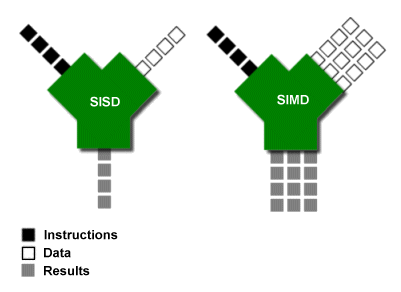
\includegraphics [width =0.4 \textwidth ]{simd.png}
\end{figure}
\vspace{-2cm}
\titlepage
\end{frame}


\begin{frame}[t]{Tabla de contenidos}
 \scriptsize
 \tableofcontents
\end{frame}


\AtBeginSubsection[]
{
  \begin{frame}[t]{Tabla de contenidos}
    \setcounter{tocdepth}{2}
    \scriptsize
    \tableofcontents[currentsection, sectionstyle=show/shaded, subsectionstyle=show/shaded/hide]
  \end{frame}
}

% \section{Procesamiento de Señales digitales}
\subsection{Digitalización de una señal}
\begin{frame}{Señal digitalizada}
 \begin{textblock*}{\textwidth}(0.4cm,1.2cm)
  \begin{itemize}[<+->]\justifying
    \item El proceso de digitalización de una señal responde al siguiente modelo.
  \end{itemize}
  \only <2> {\centering \includegraphics[width=\textwidth]{digitalizacion-layer1.pdf} }
  \only <3> {\centering \includegraphics[width=\textwidth]{digitalizacion-layer2.pdf} }
  \only <4> {\centering \includegraphics[width=\textwidth]{digitalizacion-layer3.pdf} }
  \only <5> {\centering \includegraphics[width=\textwidth]{digitalizacion-layer4.pdf} }
  \only <6> {\centering \includegraphics[width=\textwidth]{digitalizacion-layer5.pdf} }
  \only <7> {\centering \includegraphics[width=\textwidth]{digitalizacion-layer6.pdf} }
  \only <8> {\centering \includegraphics[width=\textwidth]{digitalizacion-layer7.pdf} }
 \end{textblock*} 
 \begin{textblock*}{\textwidth}(0.4cm,6.8cm)
  \begin{itemize}[<+(1)->]\justifying
    \item La función \textit{v(t)}, es una tensión de entrada analógica.
    \item La función \textit{v'(t)}, es una función discreta, que solo cambia entre valores discretos (no contínua) a intervalos regulares, dados por la frecuencia de muestreo, y mantiene su valor durante el intervalo.
  \end{itemize} 
 \end{textblock*} 
\end{frame}

\begin{frame}{Señal digitalizada}
 \begin{textblock*}{\textwidth}(0.4cm,1.2cm)
  \begin{itemize}[<+->]\justifying
   \item El circuito de Muestreo y Retención sostiene durante todo el intervalo de muestreo el valor de la señal de entrada al inicio de dicho intervalo, ignorando los demás valores.
   \item De este modo actúa sobre la variable independiente de la señal de entrada, en nuestro caso el tiempo, convirtiéndola de continua a discreta, ya que define un conjunto finito de valores de tiempo que resultan de interés.
   \item El proceso de Cuantificación (o Cuantización), transforma los valores obtenidos de la variable dependiente aproximándolos al valor mas cercano de un conjunto finito de $2^{n}$ números.
   \item A continuación mas detalles\dots
  \end{itemize} 
 \end{textblock*} 
\end{frame}

\begin{frame}{1er. Fase: Muestreo y retención}
 \begin{textblock*}{0.5\textwidth}(0.3cm,1.3cm)
  \centering
  \includegraphics[width=\textwidth]{SandH.pdf}\\ \vspace{-0.3cm}
  \only <1> {\includegraphics[width=\textwidth]{SampleAndHold-layer1.pdf} }
  \only <2-> {\includegraphics[width=\textwidth]{SampleAndHold-layer2.pdf} }
 \end{textblock*}
 \begin{textblock*}{0.5\textwidth}(0.3cm+0.5\textwidth,1.0cm)
  \begin{itemize}[<+->]\justifying
   \item Se toma un valor instantáneo de la señal y se ``retiene'' el valor de tensión en una capacidad, con un circuito resistivo de descarga de muy alta resistencia.
   \item {\textit{\color{red}Comparando la señal saliente del circuito de Muestreo y Retención, con la señal original (en punteado suave), observar que el error aumenta en los cambios abruptos de señal.}}
   \item Otra forma de observar la relación entre la frecuencia de muestreo y la máxima frecuencia de la señal original
  \end{itemize}
 \end{textblock*}
\end{frame}

\begin{frame}{Cuantificación y Codificación}
 \begin{textblock*}{0.5\textwidth}(0.3cm,1.2cm)
  \centering \vspace{-0.3cm}\includegraphics[width=\textwidth]{Cuantif.pdf}\\
  \only <4-> { \vspace{-0.8cm}\includegraphics[width=\textwidth]{Cuantif-error.pdf} }
 \end{textblock*}
 \begin{textblock*}{0.5\textwidth}(0.3cm+0.5\textwidth,1.2cm)
  \begin{itemize}[<+->]\justifying
   \item Se llevan a cabo en un Conversor Analógico Digital.
   \item Se puede aproximar por redondeo o truncamiento
   \item Independientemente del método el error aumenta en las zonas donde la derivada de la señal es mas alta.
   \item Si tomamos la diferencia entre la señal muestreada y la cuantificada y operamos una diferencia se obtiene el error de Cuantificación o Cuantización)
  \end{itemize}
 \end{textblock*}
\end{frame}

\subsection{Arquitecturas de Procesamiento de una señal digital}
\begin{frame}{Procesador de Señales Digitales}
 \begin{textblock*}{\textwidth}(0.4cm,1.2cm)
  \begin{itemize}[<+(1)->]\justifying
   \item Es una CPU de propósito dedicado, diseñada para realizar cálculos y procesamiento de un único tipo de datos: secuencias de valores correspondientes a la codificación de las muestras de una señal de entrada.
   \item Su arquitectura está pensada para optimizar el procesamiento de datos que no son de gran tamaño (8, 16, 24, o a lo sumo 32 bis). Se trata de pixeles de una imagen, o de valores instantáneos de audio, o de señales médicas o de mapas térmicos, etc.
   \item La característica distintiva de este tipo de datos reside en sus algoritmos de cálculo: Normalmente se requiere procesar no solo el valor actual sino la combinación del valor actual con n valores anteriores en el tiempo, o vecinos (en el caso de una imagen lo que llamaremos N8)
  \end{itemize}
 \end{textblock*}
\end{frame}

\begin{frame}{Procesador de Señales Digitales}
 \begin{textblock*}{\textwidth}(0.4cm,1.2cm)
  \begin{itemize}[<+(1)->]\justifying
   \item En general una operación muy frecuente son los filtros de convolución, dados por una expresión del tipo:\\
$\displaystyle y[n] = \sum_{i=0}^{N} \; a_{n}\cdot x[n-i] = a_{0}\cdot x[n] + a_{1}\cdot x[n-1] + a_{2}\cdot x[n-2] + ...  + a_{N}\cdot x[n-N]$
   \item En general se deben resolver sumas de productos y acumular su resultado.
   \item Para optimizar se deberían leer y procesar varios datos en paralelo
   \item Las técnicas de paralelismo que se desarrollaron en estos procesadores se denominaron por tal razón \textbf{\textit{\color{blue}Data Level Paralelism}}.
  \end{itemize}
 \end{textblock*}
\end{frame}

\begin{frame}{Arquitectura de un Procesador de Señales Digitales}
 \begin{textblock*}{\textwidth}(0.4cm,1.2cm)
  \begin{itemize}[<+(1)->]\justifying
   \item En general el diseño de un Procesador de Señales Digitales concentra sus esfuerzos en resolver en paralelo:
   \begin{description}[<+(1)->]\justifying
    \item[El acceso a los operandos] Para este fin se implementan buses paralelos con una cantidad de líneas de datos superior al ancho de palabra de la CPU
    \item[El almacenamiento de resultados] Se resuelve mediante buses dedicados para manejar la salida de la ALU hacia memoria o registros (con las consideraciones que la concurrencia de accesos debe tener en cuenta en el hardware)
    \item[El procesamiento de la mayor cantidad de datos posible] Los primeros pasos se conocen como VLIW (Very Large Instruction Word), que derivó en el modelo de ejecución SIMD (Single Instruction Multiple Data)
   \end{description}
  \end{itemize}
 \end{textblock*}
\end{frame}

\section {Modelo de ejecución SIMD}
\subsection{¿Por qué una unidad SIMD?}

\begin{frame}{Limitaciones del procesamiento escalar}
 \begin{textblock*}{\textwidth}(0.4cm,1.2cm) \justifying
  \only<1->{
   \begin{tcolorbox}[enhanced jigsaw,rounded corners, drop fuzzy shadow=ShadowColor]
    Durante muchos años los procesadores incrementaron su rendimiento aumentando la frecuencia de reloj y explotando el paralelismo a nivel de instrucciones (\emph{Instruction Level Parallelism, ILP}). Sin embargo, numerosas aplicaciones como procesamiento de imágenes, audio, video y señales digitales presentan una gran cantidad de operaciones idénticas sobre conjuntos extensos de datos.
   \end{tcolorbox}
   }
 \vspace{-0.3cm}
 \only<2->{
  \begin{tcolorbox}[enhanced jigsaw,rounded corners, drop fuzzy shadow=ShadowColor]
   En estos casos, ejecutar una instrucción por cada elemento resulta poco eficiente, aun cuando el procesador sea superescalar y pueda ejecutar varias instrucciones simultáneamente. Aun operaciones elementales como la suma.
  \end{tcolorbox}
 }
 \vspace{-0.6cm}
 \only<3->{
 \begin{center}
  \begin{tabular}{c}
$a_0+b_0$\\
$a_1+b_1$\\
$a_2+b_2$\\
$a_3+b_3$
  \end{tabular}
 \end{center}
 \vspace{-0.3cm}
 \textbf{\textit{\centering Cada suma requiere una instrucción independiente.}}
 }
 \end{textblock*}
\end{frame}

\begin{frame}{Procesamiento SIMD}
 \begin{textblock*}{\textwidth}(0.4cm,1.2cm) \justifying
  \only<1->{
   \begin{tcolorbox}[enhanced jigsaw,rounded corners, drop fuzzy shadow=ShadowColor]
    Las aplicaciones multimedia presentan un elevado paralelismo a nivel de datos (\emph{Data Level Parallelism, DLP}), ya que la misma operación suele aplicarse sobre grandes arreglos o vectores.
   \end{tcolorbox}
   }
 \vspace{-0.3cm}
\only<2->{
  \begin{tcolorbox}[enhanced jigsaw,rounded corners, drop fuzzy shadow=ShadowColor]
   Las arquitecturas SIMD (\emph{Single Instruction Multiple Data}) permiten que una única instrucción opere simultáneamente sobre varios elementos almacenados en un registro ancho, reduciendo el número de instrucciones ejecutadas y aumentando el rendimiento.
  \end{tcolorbox}
  }
%  \vspace{0.5cm}
 \only<3->{
  \begin{center}
   \[
    \left[
     \begin{array}{cccc}
      a_0&a_1&a_2&a_3
     \end{array}
    \right]
     +
    \left[
     \begin{array}{cccc}
      b_0&b_1&b_2&b_3
     \end{array}
    \right]
    \longrightarrow
    \left[
     \begin{array}{cccc}
      c_0&c_1&c_2&c_3
     \end{array}
    \right]
   \]
  \end{center}
  \textbf{\textit{\centering Una única instrucción produce cuatro resultados en paralelo.}}
 }
 \end{textblock*}
\end{frame}

\subsection{Un modelo de paralelización}
\begin{frame}{Single Instruction Multiple Data}
 \begin{textblock*}{0.11\textwidth}(.3cm,1.2cm)
  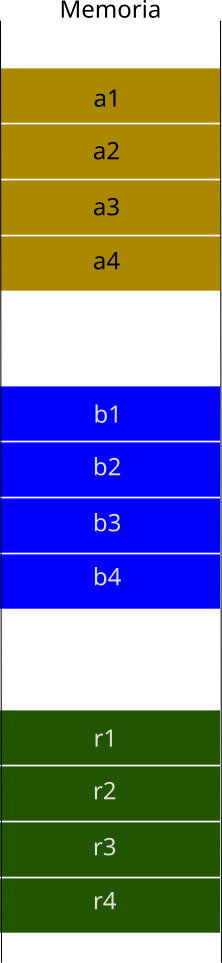
\includegraphics[width=\textwidth]{SIMD1.pdf}
 \end{textblock*}
 \begin{textblock*}{0.88\textwidth}(.14\textwidth,1.2cm)
  \begin{itemize}[<+(1)->]\justifying
   \item Se trata de un modelo de ejecución capaz de computar una sola operación sobre un conjunto de múltiples datos.
   \item Se refiere a esta técnica como paralelismo a nivel de datos.
   \item Es particularmente útil para procesar audio, video, o imágenes en donde se aplican algoritmos repetitivos sobre sets de datos del mismo formato y que se procesan en conjunto, como por ejemplo en filtros, compresores, codificadores en donde la salida depende de los últimos \textit{n} valores de muestras tomados.
   \item La figura muestra el layout típico de variables memoria para aplicar este modelo
  \end{itemize}
 \end{textblock*}
\end{frame}

\begin{frame}{Como sería la vida sin SIMD?}
 \begin{textblock*}{0.11\textwidth}(.3cm,1.2cm)
  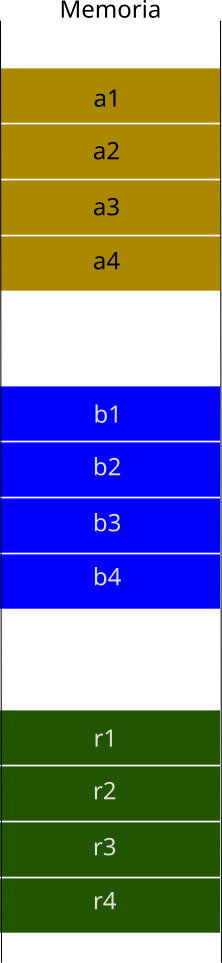
\includegraphics[width=\textwidth]{SIMD1.pdf}
 \end{textblock*}
 \begin{textblock*}{0.89\textwidth}(.11\textwidth,1.2cm)
  \begin{itemize}[<+(1)->]\justifying
   \item En contraposición a SIMD el modelo previo es SISD (\textbf{S}ingle \textbf{I}nstruction \textbf{S}ingle \textbf{D}ata)
   \item Considerando el sector de memoria de la figura, nos proponemos realizar una operación aritmética o lógica sobre las cadenas de datos $a_{n}$ y $b_{n}$, almacenando el resultado en $r_{n}$
   \item Si un procesador no dispone de un modelo arquitectural que le permita implementar paralelismo a nivel de datos, como SIMD,esta operación implica un loop, ya que solo puede procesar un dato por cada instrucción (SISD).
  \end{itemize}
 \end{textblock*}
\end{frame}

\begin{frame}{Single Instruction Single Data}
 \begin{textblock*}{\textwidth}(0.3cm,1.2cm)
  \centering \includegraphics[width=.4\textwidth]{SISD-Layer2.pdf}
 \end{textblock*}
\end{frame}

\begin{frame}{Single Instruction Single Data}
 \begin{textblock*}{\textwidth}(0.3cm,1.2cm)
  \centering \includegraphics[width=.4\textwidth]{SISD-Layer3.pdf}
 \end{textblock*}
\end{frame}

\begin{frame}{Single Instruction Single Data}
 \begin{textblock*}{\textwidth}(0.3cm,1.2cm)
  \centering \includegraphics[width=.4\textwidth]{SISD-Layer4.pdf}
 \end{textblock*}
\end{frame}

\begin{frame}{Single Instruction Single Data}
 \begin{textblock*}{\textwidth}(0.3cm,1.2cm)
  \centering \includegraphics[width=.4\textwidth]{SISD-Layer5.pdf}
 \end{textblock*}
\end{frame}

\begin{frame}{Single Instruction Multiple Data}
 \begin{textblock*}{\textwidth}(0.3cm,1.2cm)
  \begin{itemize}\justifying
   \item Cada Registro se carga en una sola instrucción
   \item La operación se efectúa en la segunda instrucción
  \end{itemize}
  \centering 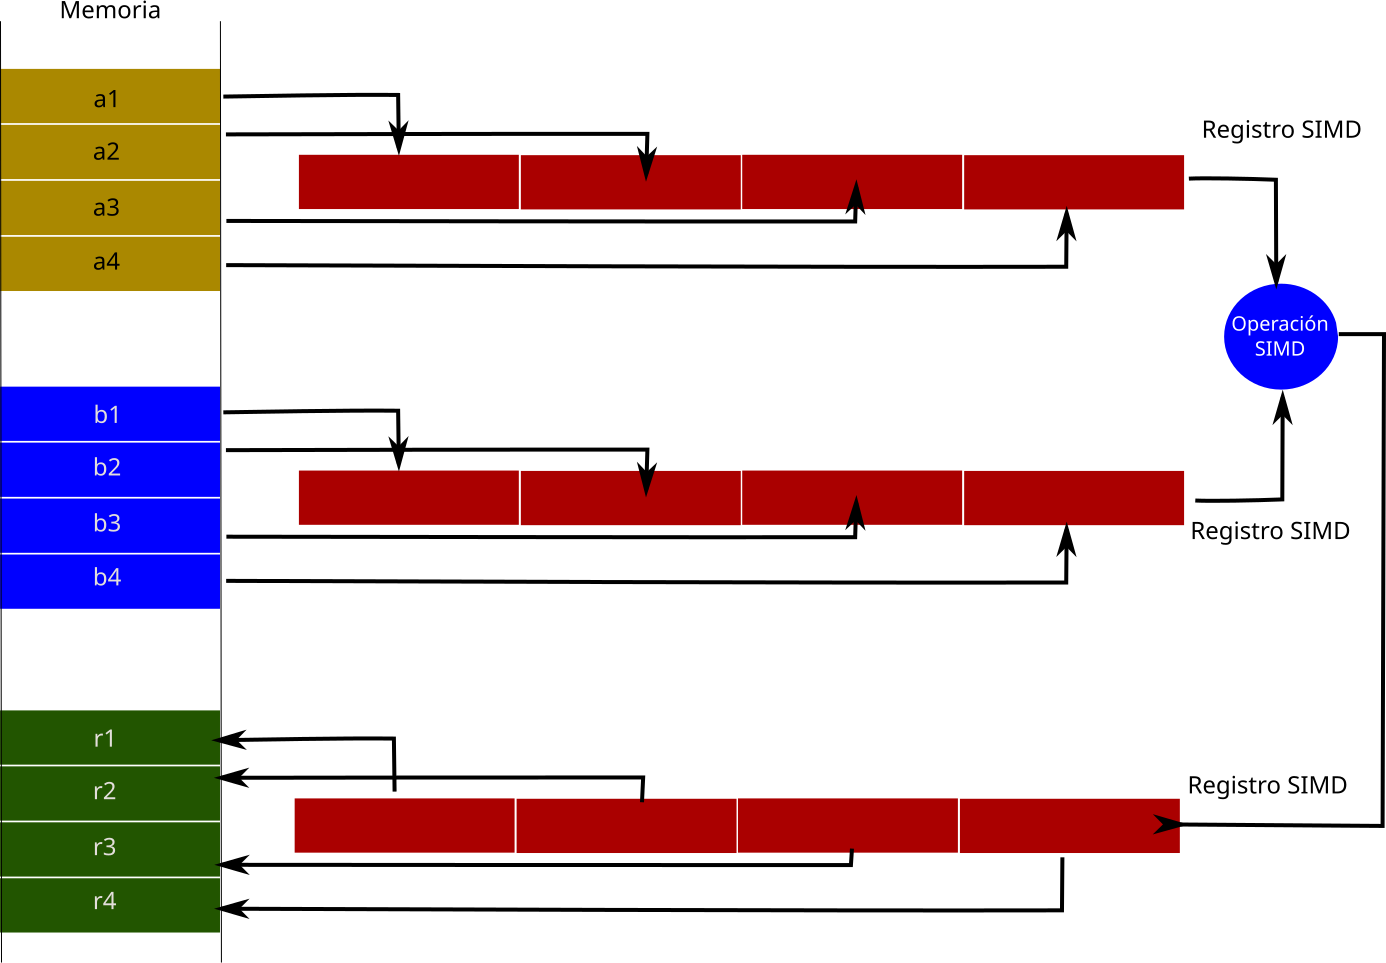
\includegraphics[width=.6\textwidth]{SIMD6.pdf}
 \end{textblock*}
\end{frame}

\begin{frame}{Resumiendo, SIMD vs. SISD}
 \begin{textblock*}{\textwidth}(0.3cm,1.2cm)
  \centering 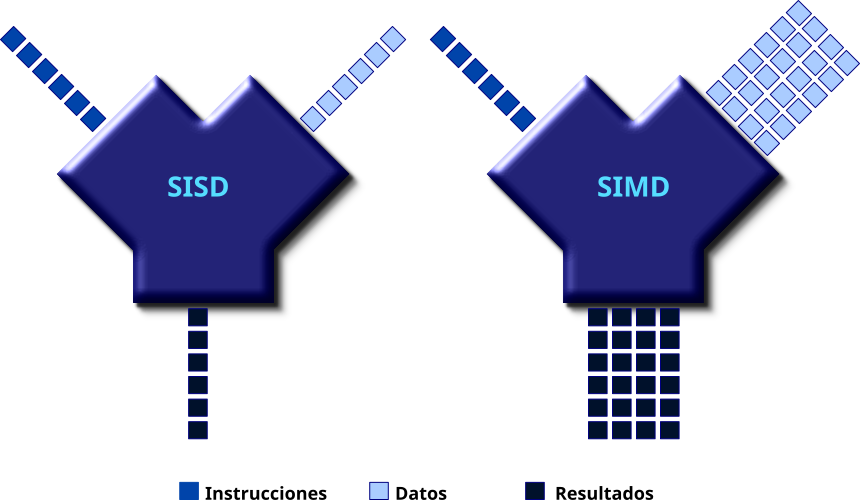
\includegraphics[width=.9\textwidth]{SISD-vs-SIMD.pdf}
 \end{textblock*}
\end{frame}

\begin{frame}{Acerca de SIMD y Procesamiento Vectorial}
 \begin{textblock*}{\textwidth}(0.4cm,1.2cm)
  \begin{tcolorbox}[enhanced jigsaw,rounded corners, drop fuzzy shadow=ShadowColor]
   \begin{itemize}[<+->]\justifying
    \item \textbf{SIMD} aplica una misma instrucción sobre un conjunto fijo de datos empaquetados en un registro ancho. Como ocurre con \textbf{NEON}.
    \item Cada registro con los que opera una instrucción \textbf{SIMD} contiene un grupo fijo de operandos empaquetados. La misma instrucción se ejecuta en paralelo sobre cada operando individual.
    \item El procesamiento vectorial opera sobre vectores de longitud variable mediante registros vectoriales y hardware capaz de recorrer automáticamente todos sus elementos.
    \item Conceptualmente, el programador ``vé'' usa loa instrucción vectorial, por ejemplo \texttt{VADD V1, V2, V3}, es decir, "sumar todos los elementos de V2 y V3 y almacenarlos en V1".
    \item Internamente el hardware ejecuta una secuencia de operaciones elementales sobre cada componente del vector, insertándolas en el pipeline.
   \end{itemize}
  \end{tcolorbox}
 \end{textblock*}
\end{frame}

\begin{frame}{Acerca de SIMD y Procesamiento Vectorial}
 \begin{textblock*}{\textwidth}(0.4cm,1.2cm)
  \begin{tcolorbox}[enhanced jigsaw,rounded corners, drop fuzzy shadow=ShadowColor]
   \begin{itemize}[<+->]\justifying
    \item La diferencia con \textbf{SIMD} es que el programador no tiene que preocuparse por cuántos elementos caben en un registro: la instrucción se aplica al vector completo, aunque el hardware lo procese en varias etapas.
    \item Dicho de otra manera:
    \begin{itemize}[<+->]\justifying
     \item \textbf{SIMD}: una instrucción opera sobre un número fijo de elementos (4, 8, 16, etc.).
     \item \textbf{Vectorial}: una instrucción opera sobre un vector de longitud arbitraria; el hardware se encarga de recorrerlo internamente.
    \end{itemize}
    \item Por eso suele decirse que los procesadores vectoriales tienen vector-length agnostic execution, mientras que \textbf{NEON} es \textbf{SIMD} de ancho fijo: \SI{128}{\bit}.
    \item \textbf{SIMD} puede interpretarse como un caso particular de procesamiento vectorial, en el que la longitud del vector coincide con el ancho fijo del registro.
    \item ARMv8 evoluciona de NEON a SVE adoptando un modelo de procesamiento vectorial de longitud variable  de hasta \SI{1024}{\bit} en pasos de \SI{128}{\bit}.
   \end{itemize}
  \end{tcolorbox}
 \end{textblock*}
\end{frame}

\section{Actualización de la arquitectura}
\subsection{Evolución de VFP y NEON}
%------------------------------------------------

\begin{frame}{Evolución de las extensiones de punto flotante y SIMD}
 \begin{textblock*}{\textwidth}(0.4cm,1.2cm)
  \begin{center} \Large
VFP $\rightarrow$ NEON $\rightarrow$ ARMv8 SIMD $\rightarrow$ SVE / SVE2
  \end{center}
  \vspace{0.5cm}
  \begin{tcolorbox}[enhanced jigsaw,rounded corners, drop fuzzy shadow=ShadowColor]
   \justifying Cada generación incorporó nuevas capacidades para mejorar el rendimiento en aplicaciones científicas, multimedia y procesamiento de señales, manteniendo compatibilidad con las generaciones anteriores.
  \end{tcolorbox}
 \end{textblock*}
\end{frame}

%------------------------------------------------

\begin{frame}[fragile]{ARMv5: aparición de VFP}
 \begin{textblock*}{\textwidth}(0.4cm,1.2cm)
  \begin{itemize}\justifying
   \item Se incorpora \textbf{VFP (Vector Floating Point)}, una unidad dedicada al procesamiento de números en punto flotante compatibles con IEEE-754.
   \item Está orientada al procesamiento \textbf{escalar}: cada instrucción opera sobre un único dato.
   \item Soporta operaciones en simple y doble precisión.
   \item Introduce un banco de registros de \SI{64}{\bit} (registros D), accesibles también como registros de \SI{32}{\bit} (registros S).
  \end{itemize}
  \vspace{0.3cm}
  \textbf{Ejemplo}
  \begin{lstlisting}[basicstyle=\scriptsize,numbers=none, escapechar=\@]
VADD.F32 S0, S1, S2
  \end{lstlisting}
  \begin{tcolorbox}[enhanced jigsaw,rounded corners, drop fuzzy shadow=ShadowColor]
   \justifying Una instrucción realiza una suma entre dos operandos escalares.
  \end{tcolorbox}
 \end{textblock*}
\end{frame}

%------------------------------------------------

\begin{frame}{ARMv6: Aparece NEON}
 \begin{textblock*}{\textwidth}(0.4cm,1.2cm)
  \begin{itemize}[<+->]\justifying \parskip 0.2cm
   \item Las aplicaciones multimedia requieren procesar múltiples datos en paralelo.
   \item ARM incorpora \textbf{NEON}, una extensión SIMD de \SI{64}{\bit} y \SI{128}{\bit}.
   \item Una única instrucción puede operar simultáneamente sobre varios enteros o números de punto flotante de simple precisión.
   \item Dependiendo del tipo de dato, una instrucción puede procesar:
   \begin{itemize}\justifying \parskip 0.2cm
    \item \SI{16}{\byte},
    \item 8 halfwords,
    \item 4 words,
    \item 2 doublewords.
   \end{itemize}
  \end{itemize}
 \end{textblock*}
\end{frame}

%------------------------------------------------

\begin{frame}{VFP y NEON}
 \begin{textblock*}{\textwidth}(0.4cm,1.2cm)
  \begin{block}{Concepto importante}\justifying
   NEON \textbf{no reemplaza} a VFP.

   Ambos constituyen conjuntos de instrucciones diferentes que comparten un mismo banco físico de registros.
  \end{block}
  \vspace{0.3cm}
  \begin{itemize}[<+(1)->]\justifying
   \item VFP está orientado al cálculo en punto flotante escalar.
   \item NEON está orientado al procesamiento SIMD.
   \item El compilador selecciona cuál utilizar según el tipo de operación.
  \end{itemize}
 \end{textblock*}
\end{frame}

%------------------------------------------------

\begin{frame}{ARMv7-A: el caso del Cortex-A9}
 \begin{textblock*}{\textwidth}(0.4cm,1.2cm)\justifying
  El Cortex-A9 integra ambas tecnologías.
  \vspace{0.3cm}
  \begin{itemize}[<+->]
   \item VFPv3.
   \item NEON.
   \item Banco de registros compartido.
   \item Tres vistas del mismo banco de registros:
   \begin{itemize}[<+->]
    \item S (32 bits),
    \item D (64 bits),
    \item Q (128 bits).
   \end{itemize}
  \end{itemize}
  \vspace{0.5cm}
  \only<8>{Este será el modelo utilizado en el resto de esta clase en particular para el procesador ARM del Zynq-7000.}
 \end{textblock*}
\end{frame}

%------------------------------------------------

\begin{frame}{ARMv8-A: unificación del modelo}
 \begin{textblock*}{\textwidth}(0.4cm,1.2cm)\justifying
  En ARMv8 desaparece la idea de un coprocesador VFP separado.
  \vspace{0.3cm}

  Existe un único banco de registros vectoriales:
  $ V0 \ldots V31$
  \vspace{0.3cm}

  Cada registro posee \SI{128}{\bit} y puede interpretarse como:
  \vspace{0.3cm}

  \begin{itemize}
   \item bytes (B),
   \item halfwords (H),
   \item words (S),
   \item doublewords (D),
   \item quadwords (Q).
  \end{itemize}
    \vspace{0.3cm}

  La arquitectura resulta más uniforme y sencilla para el compilador.
 \end{textblock*}
\end{frame}

%------------------------------------------------

\begin{frame}{SVE: Scalable Vector Extension}
 \begin{textblock*}{\textwidth}(0.4cm,1.2cm)\justifying
  NEON utiliza registros SIMD de ancho fijo (\SI{128}{\bit}).
  \vspace{0.3cm}
  SVE introduce un nuevo paradigma:
  \vspace{0.3cm}
  \begin{itemize}
   \item registros vectoriales de longitud variable;
   \item desde 128 hasta 2048 bits;
   \item múltiplos de 128 bits;
   \item el software no necesita conocer el ancho real implementado.
  \end{itemize}
  \vspace{0.3cm}
  Esto permite que un mismo programa aproveche automáticamente procesadores con registros vectoriales más anchos.
 \end{textblock*}
\end{frame}

%------------------------------------------------

\begin{frame}{SVE2}
 \begin{textblock*}{\textwidth}(0.4cm,1.2cm)\justifying

  SVE2 amplía SVE incorporando instrucciones orientadas a:

  \begin{itemize}
   \item procesamiento digital de señales (DSP);
   \item procesamiento de imágenes;
   \item códecs de audio y video;
   \item criptografía;
   \item inteligencia artificial.
  \end{itemize}

  \vspace{0.4cm}

  Puede interpretarse como una evolución de las capacidades de NEON dentro del modelo vectorial de longitud variable.
 \end{textblock*}
\end{frame}

%------------------------------------------------

\begin{frame}{¿Qué sigue vigente?}
 \begin{textblock*}{\textwidth}(0.4cm,1.2cm)\justifying
  \textbf{Para el Cortex-A9 (Zynq-7000)}
  \begin{itemize}
   \item VFPv3.
   \item NEON.
   \item Registros S, D y Q.
   \item Programación mediante ensamblador e intrinsics.
   \item Auto-vectorización de GCC y Clang.
  \end{itemize}

  \vspace{0.4cm}

  \textbf{Hacia arquitecturas modernas}

  \begin{itemize}
   \item ARMv8 unifica el banco de registros.
   \item SVE y SVE2 representan la evolución actual del procesamiento vectorial.
  \end{itemize}
 \end{textblock*}
\end{frame}


%------------------------------------------------

\section{Enfoque Práctico}

%------------------------------------------------

\begin{frame}{¿Cómo utiliza el compilador VFP y NEON?}
 \begin{textblock*}{\textwidth}(0.4cm,1.2cm)
  Cuando el programador escribe código C/C++ convencional, el compilador puede generar automáticamente instrucciones:
  \vspace{0.3cm}
  \begin{itemize}[<+(1)->]\justifying \parskip 0.2cm
   \item ARM enteras.
   \item VFP para operaciones en punto flotante.
   \item NEON para operaciones SIMD.
  \end{itemize}
  \vspace{0.4cm}
  \only<5>{
   \begin{tcolorbox}[enhanced jigsaw,rounded corners, drop fuzzy shadow=ShadowColor]
    \justifying Cuando el objetivo es aprovechar el hardware disponible prescindiendo de escribir código ensamblador, hay alternativas.
   \end{tcolorbox}
   }
 \end{textblock*}
\end{frame}

%------------------------------------------------

\begin{frame}{Tres niveles de programación}
 \begin{textblock*}{\textwidth}(0.4cm,1.2cm)
  Existen tres formas habituales de utilizar NEON.
  \vspace{0.5cm}
  \begin{enumerate}[<+(1)->]
   \item Código C/C++ convencional.
   \item Intrinsics NEON.
   \item Ensamblador.
  \end{enumerate}
  \vspace{0.5cm}
  \only<5>{
   \begin{tcolorbox}[enhanced jigsaw,rounded corners, drop fuzzy shadow=ShadowColor]
    \justifying A mayor nivel de abstracción disminuye el esfuerzo de programación, mientras que el ensamblador ofrece el máximo control sobre las instrucciones generadas.
   \end{tcolorbox}
   }
 \end{textblock*}
\end{frame}

%------------------------------------------------

\begin{frame}[fragile]{Auto-vectorización}
 \begin{textblock*}{\textwidth}(0.4cm,1.2cm)

El compilador puede detectar operaciones repetitivas sobre arreglos y generar automáticamente instrucciones SIMD.
\vspace{0.2cm}

\begin{lstlisting}[language=C,basicstyle=\scriptsize,numbers=none, escapechar=\@]
for (i=0; i<n; i++)
    c[i] = a[i] + b[i];
\end{lstlisting}

\vspace{0.2cm}

Con las opciones de optimización adecuadas, GCC o Clang pueden reemplazar el
bucle por instrucciones NEON.
 \end{textblock*}
\end{frame}

%------------------------------------------------

\begin{frame}[fragile]{Intrinsics NEON}
 \begin{textblock*}{\textwidth}(0.4cm,1.2cm)
  \begin{tcolorbox}[enhanced jigsaw,rounded corners, drop fuzzy shadow=ShadowColor]
   \justifying Los \emph{intrinsics} son funciones de C que representan casi directamente una instrucción NEON.
  \end{tcolorbox}

  \vspace{0.3cm}

  \begin{lstlisting}[language=C,basicstyle=\scriptsize,numbers=none, escapechar=\@]
uint8x16_t va, vb, vc;

vc = vaddq_u8(va, vb);
  \end{lstlisting}

  \vspace{0.3cm}
  El compilador traduce esta llamada a la instrucción NEON correspondiente, sin necesidad de recurrir a un archivo fuente adicional con código assembler.
 \end{textblock*}
\end{frame}

%------------------------------------------------

\begin{frame}{¿Cuándo utilizar intrinsics?}
 \begin{textblock*}{\textwidth}(0.4cm,1.2cm)\justifying
  Los intrinsics permiten:
  \vspace{0.5cm}
  \begin{itemize}[<+(1)->]\parskip 0.2 cm
   \item Obtener un mayor control sobre el código generado.
   \item Acceder a instrucciones específicas de NEON.
   \item Mantener la portabilidad entre compiladores compatibles.
  \end{itemize}
  \vspace{0.4cm}
  \only<5>{En la mayoría de las aplicaciones representan el mejor compromiso entre rendimiento y facilidad de mantenimiento.}
 \end{textblock*}
\end{frame}

%------------------------------------------------

\begin{frame}{¿Y el ensamblador?}
 \begin{textblock*}{\textwidth}(0.4cm,1.2cm) \justifying
  El lenguaje ensamblador sigue siendo útil cuando:
  \vspace{0.4cm}
  \begin{itemize}[<+(1)->]\parskip 0.2 cm
   \item se requiere el máximo rendimiento;
   \item se desea controlar exactamente las instrucciones emitidas;
   \item es necesario aprovechar características muy específicas del hardware.
  \end{itemize}
  \vspace{0.4cm}
  \only<5>{Sin embargo, con el transcurrir del tiempo los compiladores perfeccionaron el uso de \emph{intrinsics}, con lo cual la utilización de ensamblador es menos frecuente.}
 \end{textblock*}
\end{frame}

\section{Implementación SIMD en ARM}
\subsection{SISD, Procesamiento Vectorial, Procesamiento empaquetado}

% \begin{frame}[fragile]{Introducción}
%  \begin{textblock*}{\textwidth}(0.4cm,1.2cm)
%  \justifying
%   \only<2->{Los dos últimos gráficos, se traducen muy fácilmente en instrucciones de ARM:}
%  \end{textblock*}
%  \begin{textblock*}{.25\textwidth}(0.4cm,1.8cm)
%   \begin{onlyenv}<3->
%    \begin{tcolorbox}[enhanced jigsaw,rounded corners, drop fuzzy shadow=ShadowColor]
%     \textbf{SISD}\vspace{-0.4cm}
%     \begin{lstlisting}[basicstyle=\scriptsize,numbers=none]
% add  r0,r5
% add  r1,r6
% add  r2,r7
% add  r3,r8
%     \end{lstlisting}
%    \end{tcolorbox}
%   \end{onlyenv}
%  \end{textblock*}
%  \begin{textblock*}{.75\textwidth}(0.4cm+.25\textwidth,1.8cm)
%   \begin{onlyenv}<4->
%    \begin{tcolorbox}[enhanced jigsaw,rounded corners, drop fuzzy shadow=ShadowColor]
%     \textbf{SIMD (Modo empaquetado)}\vspace{-0.4cm}
%     \begin{lstlisting}[basicstyle=\scriptsize,numbers=none, escapechar=\@]
% VADD.I32 Q10, Q8, Q9
% // Una suma de dos registros de @\color{Gray}\SI{128}{\bit}@,
% // Cada v@\color{Gray}\'i@a de @\color{Gray}\SI{32}{\bit}@ de los registros se suma por separado.
% // No hay carry entre las v@\color{Gray}\'i@as.
%     \end{lstlisting}
%    \end{tcolorbox}
%   \end{onlyenv}
%  \end{textblock*}
%  \begin{textblock*}{\textwidth}(0.4cm,4.8cm)
%   \begin{itemize}[<+(4)->]\justifying
%    \item En ARMv5 se introducen las extensiones \textbf{VFP} (Por\textbf{V}irtual \textbf{F}loating \textbf{P}oint)
%    \item \textbf{VFP} se implementó como una unidad de punto flotante compatible con IEEE-754. Su File Register estaba compuesto por 16 registros de \SI{64}{\bit}: \textbf{\texttt{D0-D15}}, que podían interpretarse como registros de \SI{32}{\bit} \textbf{\texttt{S0-S31}}.
%    \item Las versiones posteriores ampliaron la cantidad de registros de \SI{64}{\bit} y, con ARMv7 Cortex A y R, \textbf{VFPv3} y \textbf{NEON}implementan un banco de registros compartido que puede verse como registros \textbf{\texttt{S\textsubscript{n}}}, \textbf{\texttt{D\textsubscript{n}}} o \textbf{\texttt{Q\textsubscript{n}}} según el tipo de operación.
%   \end{itemize}
%  \end{textblock*}
% \end{frame}



% \begin{frame}[fragile]{Introducción}
%  \begin{textblock*}{\textwidth}(0.4cm,1.2cm)
%   \begin{itemize}[<+->]\justifying
%    \item Hasta ARMv6 las instrucciones punto flotante se comportaban como un modelo vectorial, ejecutando una secuencia de operaciones que involucran un grupo de registros (cantidad definida en un registro de configuración). Ejemplo:
%   \end{itemize}
%   \begin{onlyenv}<2->
%    \begin{tcolorbox}[enhanced jigsaw,rounded corners, drop fuzzy shadow=ShadowColor]
%     \textbf{SIMD (Modo Vector) (Obsoleto)} \vspace{-0.4cm}
%     \begin{lstlisting}[basicstyle=\scriptsize,numbers=none, escapechar=\@]
% VADD.F32 S24, S8, S16
% // Se ejecutan cuatro operaciones:
% // S24 = S8 + S16
% // S25 = S9 + S17
% // S26 = S10 + S18
% // S27 = S11 + S19
%     \end{lstlisting}
%    \end{tcolorbox}
%   \end{onlyenv}
%   \begin{itemize}[<+(1)->]\justifying
%    \item SIMD no es una secuencia, sino una única operación. Por eso en ARMv7 las operaciones vectoriales de punto flotante se reemplazan por SIMD empaquetadas del slide anterior. Es decir NEON.
%    \item ARMv8, extiende NEON y lo mantiene compatible con ARMv7 A y R.
%   \end{itemize}
%  \end{textblock*}
% \end{frame}

\subsection{Implementación SIMD ARMv7 A y R}
\begin{frame}{Cuestiones de Implementación}
 \begin{textblock*}{\textwidth}(0.4cm,1.1cm)
  \begin{itemize}[<+->]\justifying
   \item ARM no garantiza que todos los cores incluyan NEON y VFP. Podemos encontrarnos con procesadores ARM que incluyan una de las dos o las dos.
   \item Si un core incluye NEON, pero no incluye VFP, no puede ejecutar instrucciones de punto flotante en hardware.
   \item Al ser NEON mas eficiente en el calculo vectorial, las instrucciones vectoriales de las VFP se discontinúan en los cores v7 con NEON incluido. Por tal razón la documentación técnica de ARM a menudo se refiere a la VFP como FPU (Por Floating Point Unit).
   \item El soporte a Half-Presicion y Multiplicación-Suma Fusionada depende de cada implementación de core.
   \item Una misma instrucción varía su tiempo de ejecución dependiendo del core en el que se implementa, y aun en el mismo core  depende de la cacheabilidad lograda con los datos con que se opera.
  \end{itemize}
 \end{textblock*} 
\end{frame}

\begin{frame}[fragile]{Cuestiones de Implementación}
 \begin{textblock*}{\textwidth}(0.4cm,1.1cm)
  \begin{itemize}[<+->]\justifying
   \item NEON y VFP comparten algunas instrucciones. Se las llama Shared Instructions.
   \item Si el core soporta ambas extensiones, los registros de ambas se solapan, las instrucciones VFP se ejecutan en la unidad de hardware de la VFP, pero las Shared, se ejecutan en el pipeline de Punto Flotante de NEON cuya eficiencia es mayor.
   \item VFP y NEON ejecutan en el espacio de instrucciones de los coprocesadores CP10 y CP11.
   \item VFP implementa operaciones de punto flotante 100\% compatibles con IEEE-754, precisión simple. Dependiendo de la implementación puede soportar doble precisión.
   \item NEON procesa en una sola instrucción datos enteros o punto flotante precisión simple empaquetados. En este último caso no se asegura compatibilidad completa con IEEE-754. No opera en doble precisión.
  \end{itemize}
 \end{textblock*} 
\end{frame}

\begin{frame}{Cuestiones de Implementación}
 \begin{textblock*}{\textwidth}(0.4cm,1.1cm)
  \begin{itemize}[<+->]\justifying
   \item Half-Precision solo esta soportado por una extensión específica core dependiente.
   \item Si están las extensiones Half-Precision presentes en el core, entonces tanto VFP como NEON manejarán ese tipo de datos y disponen de instrucciones de conversión de Single a Half Precision.
   \item NEON soporta operaciones de Suma de productos (Fused Multiply-Add) se soportan mediante una extensión core dependiente.
   \item Estas operaciones implican en una misma instrucción productos y acumulaciones con un solo paso de redondeo. Es de esperar una pérdida de precisión.
   \item Si NEON y VFP no se habilitan en el Registro CPACR del coprocesador CP15, cualquier instrucción generará una excepción Undefined Instruction.
  \end{itemize}
 \end{textblock*} 
\end{frame}

\subsection{Tecnología NEON}
\begin{frame}{Cuestiones de Implementación}
 \begin{textblock*}{\textwidth}(0.4cm,1.1cm)
  \begin{itemize}[<+->]\justifying
   \item ARMv7 es una arquitectura de \SI{32}{\bit}, sin embargo NEON implementa registros de \SI{64}{\bit} y \SI{128}{\bit}
   \item Los componentes de hardware de una unidad NEON son:
   \begin{itemize}[<+->]\justifying
    \item Registros NEON
    \item Un pipeline dedicado para operaciones de datos enteros empaquetados.
    \item Un pipeline dedicado para operaciones de datos en Punto Flotante Precisión Simple empaquetados.
    \item Un pipeline dedicado para operaciones load/store y permutación de datos empaquetados.
   \end{itemize}
   \item Las instrucciones NEON y las Floating Point comparten el mismo pack de registros (slides siguientes).
   \item De acuerdo con el tipo de instrucción la visión de esos registros es como registros de \SI{32}{\bit}, \SI{64}{\bit}, o \SI{128}{\bit}.
   \item Un registro NEON contiene un \textit{vector de elementos}, del mismo \textit{tipo de datos}. Cada contenedor de dato individual se llama \textit{lane}.
  \end{itemize}
 \end{textblock*} 
\end{frame}

\begin{frame}{Cuestiones de Implementación}
 \begin{textblock*}{\textwidth}(0.4cm,1.1cm)
  \begin{itemize}[<+->]\justifying
   \item Cada instrucción NEON consiste de \textit{n} operaciones que ocurren en paralelo, donde \textit{n}, es el número de \textit{lanes} en que está dividido cada vector de entrada.
   \item Cada una de las \textit{n} operaciones ocurren dentro del \textit{lane}, es decir no hay posibilidad de carry ni overflow de un \textit{lane} al siguiente.
  \end{itemize}
 \end{textblock*} 
  \begin{textblock*}{.5\textwidth}(0.4cm,3.7cm)
  \begin{onlyenv}<3->
   \begin{tcolorbox}[enhanced jigsaw,rounded corners, drop fuzzy shadow=ShadowColor]
    Vector NEON de \SI{64}{\bit}\\
%     \begin{itemize}
     - Ocho Elementos de \SI{8}{\bit}\\
     - Cuatro Elementos de \SI{16}{\bit}\\
     - Dos Elementos de \SI{32}{\bit}\\
     - Un Elementos de \SI{64}{\bit}  
%     \end{itemize}
   \end{tcolorbox}
  \end{onlyenv} 
 \end{textblock*}
 \begin{textblock*}{.5\textwidth}(0.4cm+.5\textwidth,3.7cm)
  \begin{onlyenv}<4->
   \begin{tcolorbox}[enhanced jigsaw,rounded corners, drop fuzzy shadow=ShadowColor]
    Vector NEON de \SI{128}{\bit}\\
%     \begin{itemize}
     - Dieciséis Elementos de \SI{8}{\bit}\\
     - Ocho Elementos de \SI{16}{\bit}\\
     - Cuatro Elementos de \SI{32}{\bit}\\
     - Dos Elementos de \SI{64}{\bit} 
%     \end{itemize}
   \end{tcolorbox}
  \end{onlyenv} 
 \end{textblock*}
\end{frame}

\begin{frame}{Cuestiones de Implementación}
\begin{textblock*}{\textwidth}(0.4cm,1.3cm)
  \centering 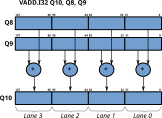
\includegraphics[width=0.6\textwidth]{Neon-vadd-i32.pdf}
 \end{textblock*} 
\end{frame}

\begin{frame}{Solapamiento de Registros}
 \begin{textblock*}{\textwidth}(0.4cm,1.2cm) \justifying
  \only<1>{La extensión VFPv2, introduce 32 registros de \SI{32}{\bit} para almacenar números en Punto Flotante Simple Precisión en formato IEEE-754. Solo accesibles con VFP.\\ \vspace{-0.3cm}
  \begin{center} \includegraphics[width=0.5\textwidth]{VFP-Registers-layer1.pdf}\end{center}}
  \only<2>{VFPv2 los agrupa en 16 registros de \SI{64}{\bit}, para almacenar números en Punto Flotante doble precisión IEEE-754. Solo accesibles con VFPv2\\ \vspace{-0.3cm}
  \begin{center} \includegraphics[width=0.5\textwidth]{VFP-Registers-layer2.pdf}\end{center}}
  \only<3>{La VFPv-3 agrega otros 16 registros de \SI{64}{\bit}, para Punto Flotante doble precisión y para datos empaquetados en las Extensiones avanzadas SIMD (NEON).\\ \vspace{-0.3cm}
  \begin{center} \includegraphics[width=0.5\textwidth]{VFP-Registers-layer3.pdf}\end{center}}
  \only<4>{Las Extensiones avanzadas NEON pueden trabajar con datos empaquetados de \SI{128}{\bit} agrupando los 32 registros de \SI{64}{\bit} en 16 registros de \SI{128}{\bit}. Solo accesible con NEON.\\ \vspace{-0.3cm}
  \begin{center} \includegraphics[width=0.5\textwidth]{VFP-Registers-layer4.pdf}\end{center}}
 \end{textblock*} 
\end{frame}

\subsection{Tipos de datos}
\begin{frame}{Escalares}
 \begin{textblock*}{\textwidth}(0.4cm,1.2cm)
  \only<1->{
   \begin{tcolorbox}[enhanced jigsaw,rounded corners, drop fuzzy shadow=ShadowColor]
    Un escalar se refiere a un valor simple de 8, 16, 32, o \SI{64}{\bit} en lugar de un vector con múltiples valores de cualquiera de estos tipos empaquetados en lanes.\\
    Se lo accede utilizando el número de lane como índice dentro del vector.
   \end{tcolorbox}
   }
 \end{textblock*} 
 \begin{textblock*}{\textwidth}(0.4cm,3.3cm)
   \only<2->{ \begin{center} 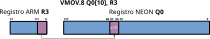
\includegraphics[width=0.95\textwidth]{Neon-scalar.pdf}\end{center} }
 \end{textblock*} 
 \begin{textblock*}{\textwidth}(0.4cm,6.5cm)
  \only<3->{
   \begin{tcolorbox}[enhanced jigsaw,rounded corners, drop fuzzy shadow=ShadowColor]
    Para instrucciones de multiplicación solo trabaja con escalares de 16 o \SI{32}{\bit}.\\
    - Escalares de \SI{16}{\bit} solo para D0[x]-D7[x], con $0 \leq x \leq 3$ \\
    - Escalares de \SI{32}{\bit} solo para D0[x]-D15[x], para x 0 ó 1.
   \end{tcolorbox}
   }
 \end{textblock*} 
\end{frame}

\begin{frame}{Tipos de Datos}
 \begin{scriptsize}
  \begin{center}
   \begin{textblock*}{\textwidth}(0.4cm,1.2cm)
    \begin{tikzpicture}
     \node (tbl) { 
      \rowcolors[]{1}{}{gray!5}
      \begin{tabularx}{.8\textwidth}{p{.25\textwidth} p{.12\textwidth} p{.12\textwidth} p{.12\textwidth} p{.12\textwidth} }
       \textbf{\color{white} } & \textbf{\color{white} \SI{8}{bit}} & \textbf{\color{white} \SI{16}{bit}} & \textbf{ \color{white}\SI{32}{bit}} & \textbf{ \color{white}\SI{64}{bit}}\\
       Unsigned integer & U8 & U16 & U32 & U64\\
       Signed integer & S8 & S16 & S32 & S64\\
       Integer (Tipo no especificado) & I8 & I16 & I32 & I64\\
       Floating-point & NA & F16 & F32 or F & NA\\
       Polynomial over \{0,1\} & P8 & P16 & NA & NA\\
      \end{tabularx}
     };
     \begin{pgfonlayer}{background}
      \draw[rounded corners,top color=red,bottom color=black,draw=white] ($(tbl.north west)+(0.14,0)$) rectangle ($(tbl.north east)-(0.13,0.45)$);
      \draw[rounded corners,top color=white,bottom color=black, middle color=red,draw=blue!20] ($(tbl.south west)+(0.12,0.5)$) rectangle ($(tbl.south east)-(0.12,0)$);
      \draw[top color=blue!1,bottom color=blue!20,draw=white] ($(tbl.north east)-(0.13,0.6)$) rectangle ($(tbl.south west)+(0.13,0.2)$);
     \end{pgfonlayer}
    \end{tikzpicture}
   \\Tipos de Datos NEON\\
   \end{textblock*} 

   \begin{textblock*}{\textwidth}(0.4cm,4.2cm)
    \begin{tikzpicture}
     \node (tbl) { 
      \rowcolors[]{1}{}{gray!5}
      \begin{tabularx}{0.6\textwidth}{p{.2\textwidth} p{.1\textwidth} p{.11\textwidth} p{.1\textwidth} }
       \textbf{\color{white} } & \textbf{\color{white} \SI{16}{bit}} & \textbf{ \color{white}\SI{32}{bit}} & \textbf{ \color{white}\SI{64}{bit}}\\
       Unsigned integer & U16 & U32 & NA\\
       Signed integer & S16 & S32 & NA\\
       Floating-point & F16 & F32 o F & F64 o D\\
      \end{tabularx}
     };
     \begin{pgfonlayer}{background}
      \draw[rounded corners,top color=red,bottom color=black,draw=white] ($(tbl.north west)+(0.14,0)$) rectangle ($(tbl.north east)-(0.13,0.45)$);
      \draw[rounded corners,top color=white,bottom color=black, middle color=red,draw=blue!20] ($(tbl.south west)+(0.12,0.5)$) rectangle ($(tbl.south east)-(0.12,0)$);
      \draw[top color=blue!1,bottom color=blue!20,draw=white] ($(tbl.north east)-(0.13,0.6)$) rectangle ($(tbl.south west)+(0.13,0.2)$);
     \end{pgfonlayer}
    \end{tikzpicture}
   \\Tipos de Datos VFP
   \end{textblock*} 
  
  \end{center}
 \end{scriptsize}
\end{frame}
\subsection{Activación}
\begin{frame}[fragile]{Habilitación de NEON y VFP}
 \begin{textblock*}{\textwidth}(0.4cm,1.3cm)
  \begin{tcolorbox}[enhanced jigsaw,rounded corners, drop fuzzy shadow=ShadowColor]
El Registro de Control de Acceso del CP15, es donde se habilitan los coprocesadores CP0 a CP13. En particular necesitamos activar CP10 y CP11, para tener disponibles los recursos SIMD y VFP.
  \end{tcolorbox}
  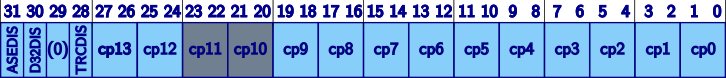
\includegraphics[width=\textwidth]{CPACR.pdf}
 \end{textblock*} 
 \begin{textblock*}{\textwidth}(0.4cm,5.6cm)
  \begin{onlyenv}<2->  
   \begin{lstlisting}[basicstyle=\scriptsize,numbers=none, escapechar=\@]
MRC p15,0,r0,c1,c0,2    // Lee CPACR de cp15 (Access Control Register). 
ORR r0,r0,#0x00f00000   // Pone NEON/VFP accesibles. Habilita cp10 y cp11 CPACR[23-20]
MCR p15,0,r0,c1,c0,2    // Escribe CPACR (Habilita NEON).
ISB                     // Instruction Syncronization Barrier: flush pipeline, y refetch.
MOV r0,#0x40000000      // Enciende hardware VFP y NEON.
MSR FPEXC,r0            // Setea bit EN en FPEXC
   \end{lstlisting}
  \end{onlyenv} 
 \end{textblock*} 
\end{frame}

\section{Microarquitectura NEON}

\subsection{Cortex A8}
\begin{frame}{NEON en el procesador Cortex A8}
 \begin{textblock*}{\textwidth}(0.4cm,1.2cm)
  \begin{tcolorbox}[enhanced jigsaw,rounded corners, drop fuzzy shadow=ShadowColor]
   El Cortex-A8 es el primer miembro de la familia ARMv7A. Es mas complejo que los procesadores ARM presentados previamente.\\
   Incluye dos pipelines simétricos para instrucciones enteras de 13 etapas, con ejecución de instrucciones en orden, y un pipeline de 10 etapas para instrucciones NEON y de Punto Flotante (VFP), sobre regstros de 64 y 128 bits.\\
   Soporta VFPv3 y Jazzele RCT.
  \end{tcolorbox}
 \end{textblock*}
\end{frame}
%
% \begin{frame}{NEON en el procesador Cortex A8}
%  \begin{textblock*}{\textwidth}(0.4cm,1.2cm)
%   \centering 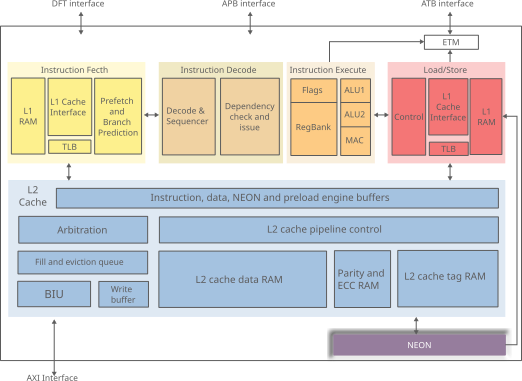
\includegraphics[width=0.65\textwidth]{CortexA8.pdf}
%  \end{textblock*}
% \end{frame}
%
% \begin{frame}{NEON en el procesador Cortex A8: El cache}
%  \begin{textblock*}{\textwidth}(0.4cm,1.2cm)
%  \only<2->{
%   \begin{tcolorbox}[enhanced jigsaw,rounded corners, drop fuzzy shadow=ShadowColor]
%    El sistema cache del Cortex A8, se compone de un cache L1 para instrucciones de \SI{16}{\kibi\byte}, un cache L1 de Datos de \SI{32}{\kibi\byte}, ambos unificados en un cache L2 de \SI{1}{\mebi\byte}.
%   \end{tcolorbox}
%   }
%  \end{textblock*}
%  \begin{textblock*}{\textwidth}(0.4cm,3.5cm)
%  \only<3->{
%   \begin{tcolorbox}[enhanced jigsaw,rounded corners, drop fuzzy shadow=ShadowColor]
%    Ambos caches L1 y L2 se vinculan al core con un Bus de Datos de \SI{128}{\bit}. El L1 está indexado virtualmente y tageado físicamente, mientras que el L2 utiliza direcciones físicas tanto para índices como para tags.
%   \end{tcolorbox}
%   }
%  \end{textblock*}
%  \begin{textblock*}{\textwidth}(0.4cm,6cm)
%  \only<4->{
%   \begin{tcolorbox}[enhanced jigsaw,rounded corners, drop fuzzy shadow=ShadowColor]
%    Los datos utilizados por la Unidad NEON por default no se almacenan en el L1. Sin embargo NEON puede leer y escribir en L1 si lo necesita.
%   \end{tcolorbox}
%   }
%  \end{textblock*}
% \end{frame}
%
% \begin{frame}{NEON en el procesador Cortex A8: MPE}
%  \begin{textblock*}{\textwidth}(0.4cm,1.2cm)
%  \only<2->{
%   \begin{tcolorbox}[enhanced jigsaw,rounded corners, drop fuzzy shadow=ShadowColor]
%    En el MPE (Media Processing Engine) el inicio de la Unidad de Ejecución Neon, se conecta a la salida del pipeline de enteros principal. Como resultado, excepciones o mal predicciones de salto pueden resolverse antes de que la instrucción los alcance.
%   \end{tcolorbox}
%   }
%  \end{textblock*}
%  \begin{textblock*}{\textwidth}(0.4cm,3.6cm)
%  \only<3->{
%   \begin{tcolorbox}[enhanced jigsaw,rounded corners, drop fuzzy shadow=ShadowColor]
%    La Unidad Entera de un Cortex A8, calcula la dirección de las instrucciones NEON de load y store a medida que pasan por el pipeline, permitiendo buscar los datos en la cache L1 antes de ser requeridos para su procesamiento por la instrucción NEON.
%   \end{tcolorbox}
%   }
%  \end{textblock*}
%  \begin{textblock*}{\textwidth}(0.4cm,6.4cm)
%  \only<4->{
%   \begin{tcolorbox}[enhanced jigsaw,rounded corners, drop fuzzy shadow=ShadowColor]
%    La profundidad adicional del pipeline NEON, junto con el buffering en la carga de datos entre la Unidad NEON, el pipeline ARM de enteros y el sistema de memoria, permite neutralizar la demora en el acceso al cache L2 (latency).
%   \end{tcolorbox}
%   }
%  \end{textblock*}
% \end{frame}
%
% \begin{frame}{NEON en el procesador Cortex A8: MPE}
%  \begin{textblock*}{\textwidth}(0.4cm,1.2cm)
%  \only<1->{
%   \begin{tcolorbox}[enhanced jigsaw,rounded corners, drop fuzzy shadow=ShadowColor]
%    En las operaciones de store se emplea un buffer de escrituras que previene de bloqueo al pipeline para instrucciones NEON de store, y detecta colisiones de direcciones entre la Unidad entera de ARM, e instrucciones NEON de load.
%   \end{tcolorbox}
%   }
%  \end{textblock*}
%  \begin{textblock*}{\textwidth}(0.4cm,3.6cm)
%  \only<2->{
%   \begin{tcolorbox}[enhanced jigsaw,rounded corners, drop fuzzy shadow=ShadowColor]
%    \textbf{NIQ}: \textbf{N}EON \textbf{I}nstruction \textbf{Q}ueue, es el desacople entre el pipeline NEON de 10 etapas, y el final del pipeline de Enteros de ARM.
%   \end{tcolorbox}
%   }
%  \end{textblock*}
%  \begin{textblock*}{\textwidth}(0.4cm,5.5cm)
%  \only<3->{
%   \begin{tcolorbox}[enhanced jigsaw,rounded corners, drop fuzzy shadow=ShadowColor]
%    La Unidad de Ejecución de Instrucciones general del pipeline le puede enviar a la Unidad NEON hasta dos instrucciones en cada ciclo de clock. La Unidad NEON envía y ejecuta una instrucción (entra o de punto flotante) por clock y la retira en orden. Excepciones y miss predictions se resuelven en la Unidad de Enteros, por lo tanto las instrucciones NEON no generan excepciones.
%   \end{tcolorbox}
%   }
%  \end{textblock*}
% \end{frame}
%
% \begin{frame}{NEON en el procesador Cortex A8: MPE}
%  \begin{textblock*}{\textwidth}(0.4cm,1.2cm)
%  La Unidad NEON de un Cortex A8 tiene:
%   \begin{itemize}[<+->] \justifying
%    \item Vías de \SI{128}{\bit} para load y store con las cache L1 y L2, como capacidad de streaming de datos.
%    \item Tres Pipelines SIMD enteros:
%    \begin{itemize}[<+->] \justifying
%     \item [\checkmark] Multiplicador Acumulador entero (MAC)
%     \item [\checkmark] Barrel Shifter de Enteros
%     \item [\checkmark] ALU entera
%    \end{itemize}
%    \item Un Pipeline de permutación de operaciones Load/Store
%    \begin{itemize}[<+->] \justifying
%     \item [\checkmark] Load/Store de datos NEON
%     \item [\checkmark] Transferencias hacia/desde la Unidad de enteros.
%     \item [\checkmark] Permutación de datos tales como entrelazado y desentrelazado.
%    \end{itemize}
%    \item Dos pipelines SIMD Punto flotante Precisión Simple
%    \begin{itemize}[<+->] \justifying
%     \item [\checkmark] Multiplicación
%     \item [\checkmark] Suma.
%    \end{itemize}
%    \item Una Unidad de punto flotante para instrucciones VFPv3 por fuera del pipeline NEON.
%   \end{itemize}
%  \end{textblock*}
% \end{frame}
%
% \begin{frame}{Procesador Cortex A8: Acceso a memoria de Datos}
%  \begin{textblock*}{\textwidth}(0.4cm,1.2cm)
%   \begin{itemize}[<+->] \justifying \parskip 0.2cm
%    \item El bit L1NEON en cp15, habilita el cache L1 para NEON. No obstante aún con este bit deshabilitado puede tenerse un hit en L1 si el dato fue accedido mediante instrucciones ARM (No NEON).
%    \item Los hazards entre datos NEON y datos del pipeline ARM se resuelven con la granularidad de las líneas de cache.
%    \item Para maximizar performance en acceso a datos:
%    \begin{itemize}[<+->] \justifying \parskip 0.2cm
%     \item [\checkmark] Evitar mezclar accesos de datos NEON y ARM dentro de la misma línea de cache.
%     \item [\checkmark] Utilizar para rutinas de copia de memoria instrucciones NEON. Se obtiene mayor performace y se evita cache pollution en el L1.
%    \end{itemize}
%    \item Ambos niveles de cache tienen \SI{64}{\byte} de tamaño, y en virtud de la profundidad del pipeline para las instrucciones NEON, por default los datos NEON se mantienen en L2.
%   \end{itemize}
%  \end{textblock*}
% \end{frame}
%
% \begin{frame}[fragile]{Procesador Cortex A8: Acceso a memoria de Datos}
%  \begin{textblock*}{\textwidth}(0.4cm,1.2cm)
%  Solo se puede admitir el envío de dos instrucciones NEON en el mismo ciclo de clock, si:
%   \begin{itemize}[<+->] \justifying \parskip 0.4cm
%    \item Instrucciones sin dependencias de datos
%    \item Una de ellas es de procesamiento y la otra se ajusta a uno de los siguientes casos
%    \begin{itemize}[<+->] \justifying  \parskip 0.4cm
%     \item [\checkmark] Es una instrucción Load/Store
%     \item [\checkmark] Es una instrucción de transferencia ARM NEON o viceversa
%     \item [\checkmark] Es una instrucción de permutación.
%    \end{itemize}
%   \end{itemize}
%  \end{textblock*}
% \end{frame}
%
% \begin{frame}[fragile]{Procesador Cortex A8: Pipeline Hazards}
%  \begin{textblock*}{\textwidth}(0.4cm,1.2cm)
%   \begin{itemize}[<+->] \justifying \parskip 0.2cm
%    \item El pipeline NEON ejecuta varias etapas luego del pipeline ARM, recibiendo de éste sus instrucciones a través de una FIFO. Las transferencias entre registros NEON y ARM es muy rápida pero el acceso a registros de coprocesadores mediante MRC desde NEON insume 20 ciclos de clock.
%    \item NEON tiene su propia Unidad Load/Store que opera en principio sin considerar el L1. Dispone de hardware para resolver accesos no ordenados a memoria. Si ambos accesos se dan en la misma línea de cache, se requieren 20 ciclos de reloj para resolverlo.
%    \item Para evitarlo se debe escribir código tratando de reducir la combinación de accesos a memoria desde ARM y NEON. En caso de ser necesario levantar desde registros ARM el resultado de un procesamiento NEON almacenado en memoria, se requieren 20 ciclos de clock.
%   \end{itemize}
%  \end{textblock*}
% \end{frame}
%
% \begin{frame}[fragile]{Procesador Cortex A8: Pipeline Hazards}
%  \begin{textblock*}{\textwidth}(0.4cm,1.2cm)
%   \begin{itemize}[<+->] \justifying \parskip 0.4cm
%    \item Una alternativa a considerar es antes del acceso resolver alguna tarea con código ARM de modo de no entrelazar los acceso a memoria. Esto generalmente funciona mejor que transferencias NEON ARM, ya que éstas pueden congestionar el pipeline.
%    \item Los compiladores utilizan una función propia para retornar un valor de punto flotante para evitar los 20 ciclos de clock de delay.
%    \item Los saltos condicionales que evalúan datos en punto flotante incurren también en esta penalidad. A pesar que la Unidad de punto flotante tiene todos los elementos para evaluar correctamente la condición. Pero retornar el resultado de la evaluación al pipeline ARM consume 20 ciclos de clock.
%   \end{itemize}
%  \end{textblock*}
% \end{frame}

\subsection{Organización física del Cortex-A9}
\begin{frame}{Arquitectura general del Cortex-A9}
 \begin{textblock*}{\textwidth}(0.4cm,1.2cm)
 \justifying El Cortex-A9 integra en un mismo core varias unidades funcionales que pueden trabajar simultáneamente para incrementar el rendimiento.
  \vspace{0.3cm}
  \begin{itemize}[<+(1)->]
   \item Front-End encargado del \textit{fetch} y decodificación de instrucciones.
   \item Pipeline entero con ejecución superescalar y fuera de orden.
   \item Unidad de Load/Store conectada a la memoria caché L1 de datos.
   \item Unidad VFP para operaciones escalares en punto flotante.
   \item Unidad NEON para operaciones SIMD sobre datos enteros y de punto flotante.
   \item Cache L1 splited para instrucciones y datos.
  \end{itemize}
  \vspace{0.4cm}
  \only<8>{En los siguientes apartados se analizará el funcionamiento interno de cada una de estas unidades.}
 \end{textblock*}
\end{frame}

\begin{frame}{Banco de registros compartido}
 \begin{textblock*}{\textwidth}(0.4cm,1.2cm)
 \justifying Las unidades VFP y NEON comparten un único banco físico de registros. Este banco puede interpretarse de tres maneras distintas:

 \vspace{0.2cm}
 \only<2->{
 \[
 \boxed{
 S_0 \ldots S_{63}
 }
 \]

 Registros de 32 bits.
 }
 \vspace{0.2cm}
 \only<3->{
 \[
 \boxed{
 D_0 \ldots D_{31}
 }
 \]

 Registros de 64 bits.
 }
 \vspace{0.2cm}
 \only<4->{
 \[
 \boxed{
 Q_0 \ldots Q_{15}
 }
 \]

 Registros SIMD de 128 bits.\\}
 \vspace{0.4cm}
 \only<5>{Lejos de ser tres bancos distintos; se trata de tres vistas del mismo conjunto físico de registros (Un solo Register File).}
 \end{textblock*}
\end{frame}

\begin{frame}{Unidad VFP}
 \begin{textblock*}{\textwidth}(0.4cm,1.2cm)
  \justifying
  La unidad \textbf{VFP} está especializada en operaciones de punto flotante compatibles con IEEE-754.
  \vspace{0.3cm}
  \begin{itemize}[<+(1)->]
   \item Opera principalmente sobre los registros $S_{n}$ y $D_{n}$.
   \item Ejecuta operaciones escalares.
   \item Implementa suma, resta, multiplicación, división, conversión y comparación en punto flotante.
   \item Comparte el Register File con NEON.
   \item Las instrucciones VFP y NEON pertenecen a conjuntos de instrucciones diferentes.
  \end{itemize}
  \vspace{0.4cm}
  \only<7>{VFP constituye la unidad de cálculo de propósito general para aplicaciones científicas y de ingeniería.}
 \end{textblock*}
\end{frame}

\begin{frame}{Unidad NEON}
 \begin{textblock*}{\textwidth}(0.4cm,1.2cm)
  \justifying La unidad \textbf{NEON} implementa una arquitectura SIMD de ancho fijo  (\SI{128}{\bit}).
  \vspace{0.3cm}
  \begin{itemize}[<+(1)->]
   \item Opera principalmente sobre registros $Q_{n}$.
   \item Cada instrucción procesa simultáneamente múltiples elementos.
   \item Soporta datos enteros de 8, 16, 32 y \SI{64}{\bit}.
   \item También admite operaciones en punto flotante de simple precisión.
   \item Está optimizada para procesamiento multimedia, DSP, imágenes y video.
  \end{itemize}
  \vspace{0.4cm}
  \only<7>{La mayor parte del incremento de rendimiento proviene del paralelismo de datos, reduciendo significativamente el número de instrucciones ejecutadas.}
 \end{textblock*}
\end{frame}

\begin{frame}{Organización Funcional del Cortex-A9}
 \begin{textblock*}{8cm}(0.3cm,1.2cm)
  \centering 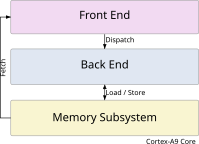
\includegraphics[width=7.8cm]{00_HiLevelView.pdf}\\
 \end{textblock*}
 \begin{textblock*}{7.2cm}(0.8cm,7.2cm)
  \justifying \scriptsize El término ``core'' se refiere al conjunto CPU + cachés locales + hardware privado asociado (ej.: el Private Timer). Utilizamos el término CPU al referirnos exclusivamente al motor de ejecución.
 \end{textblock*}
 \begin{textblock*}{7cm}(8.5cm,1.2cm) \justifying
  \only<2-> {La microarquitectura de un Cortex-A9 puede verse como tres grandes bloques:}
  \begin{itemize} \justifying
   \item<3-> Front-End: obtiene y decodifica instrucciones, analiza dependencias, renombra y despacha fuera de orden.
   \item<4-> Back-End: ejecuta las instrucciones enteras, Load/Store, VFP y NEON.
   \item<5-> Subsistema de memoria: abastece de instrucciones y datos al procesador, y recibe stores.
  \end{itemize}
  \only<6>{Este primer nivel de separación de tareas permite mantener simultáneamente ocupadas las distintas unidades funcionales, asegurando paralelismo a nivel de instrucción.}
 \end{textblock*}
\end{frame}

\begin{frame}{Front-End: Organización general}
 \begin{textblock*}{.37\textwidth}(0.3cm,1.2cm)
  \centering 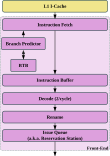
\includegraphics[width=.9\textwidth]{03_frontend.pdf}
 \end{textblock*}
 \begin{textblock*}{.6\textwidth}(.42\textwidth,1.2cm)
  \justifying  El \textbf{Front-End} prepara el flujo de instrucciones antes de su ejecución.
  \vspace{0.2cm}
  \begin{itemize} [<+(1)->]\justifying
   \item Obtiene instrucciones desde la memoria L1 I-Cache.
   \item Predice los branch procurando mantener el flujo de ejecución con mínimas interrupciones del pipeline.
   \item Decodifica las instrucciones.
   \item Analiza dependencias, y renombra los registros comprometidos en hazards.
   \item Despacha instrucciones hacia las unidades de ejecución.
  \end{itemize}
  \only<7>{El objetivo del Front-End es mantener continuamente alimentado el Back-End con instrucciones listas para ejecutar.
  }
 \end{textblock*}
\end{frame}

\begin{frame}{Front-End: problemas que debe resolver}
 \begin{textblock*}{\textwidth}(0.4cm,1.2cm)
  \begin{tcolorbox}[enhanced jigsaw,rounded corners,drop fuzzy shadow=ShadowColor]
   \begin{itemize}[<+->]\justifying
    \item Obtener un flujo continuo de instrucciones desde la memoria.
    \item Minimizar los vaciados del pipeline ocasionadas por los saltos mediante predicción dinámica.
    \item Traducir las instrucciones a operaciones internas del procesador.
    \item Eliminar dependencias falsas mediante renombrado de registros.
    \item Preparar las instrucciones para su posterior despacho hacia las unidades de ejecución.
   \end{itemize}
  \end{tcolorbox}
 \end{textblock*}
\end{frame}

\begin{frame}{¿Qué necesita un procesador con ejecución fuera de orden?}
 \begin{textblock*}{\textwidth}(0.4cm,1.2cm)
  \begin{tcolorbox}[enhanced jigsaw,rounded corners,drop fuzzy shadow=ShadowColor]
   \begin{itemize}[<+->]\justifying
    \item Asociar cada operando con la instrucción que lo producirá.
    \item Permitir que las instrucciones esperen hasta que todos sus operandos estén disponibles.
    \item Detectar cuándo una instrucción está lista para ejecutarse.
    \item Seleccionar dinámicamente instrucciones listas para su emisión.
   \end{itemize}
  \end{tcolorbox}
 \end{textblock*}
\end{frame}

\begin{frame}{Modelo conceptual del Front-End}
 \begin{textblock*}{8cm}(0.3cm,1.2cm)
 \centering
 \Large
 Fetch\\
 $\Downarrow$\\
 Decode\\
 $\Downarrow$\\
 Register Rename\\
 $\Downarrow$\\
 Instruction Queue\\
 $\Downarrow$\\
 Back-End\\
 \end{textblock*}
 \begin{textblock*}{7cm}(8.5cm,1.2cm)
 \justifying
 \only<2->{
 Este modelo resume las funciones mínimas que debe implementar un procesador superescalar con ejecución fuera de orden.\\
 }
 \vspace{0.3cm}
 \only<3->{
 Los distintos fabricantes utilizan estructuras con diferentes nombres, pero todas cumplen funciones equivalentes.\\
 }
 \vspace{0.3cm}
 \only<4->{
 Durante el resto del curso utilizaremos este modelo conceptual para comprender el funcionamiento interno del Cortex-A9.
 }
 \end{textblock*}
\end{frame}

\begin{frame}{Modelo conceptual utilizado}
 \begin{textblock*}{\textwidth}(0.4cm,1.4cm)
  \begin{tcolorbox}[enhanced jigsaw,colback=blue!4]
   \justifying
   La documentación pública del Cortex-A9 no describe completamente la organización interna de todas las estructuras utilizadas para implementar la ejecución fuera de orden.

   Emplearemos un modelo conceptual basado en los mecanismos clásicos de renombrado de registros, asociación mediante etiquetas (\textit{tags}) y emisión dinámica de instrucciones, ya que dichos mecanismos representan el fundamento de la mayoría de los procesadores superescalares modernos.
  \end{tcolorbox}
 \end{textblock*}
\end{frame}


\begin{frame}{Back-End: Organización general}
 \begin{textblock*}{8cm}(0.3cm,1.2cm)
  \centering
  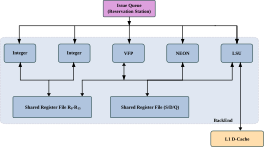
\includegraphics[width=7.8cm]{04_backend.pdf}
 \end{textblock*}
 \begin{textblock*}{7cm}(8.5cm,1.2cm)
  \justifying
  El \textbf{Back-End} recibe instrucciones desde la \textbf{Issue Queue} y es el motor de ejecución del procesador.
  \begin{itemize}[<+(1)->]\justifying
   \item La lógica de Despacho del Front-End selecciona dinámicamente las instrucciones cuyos operandos ya se encuentran disponibles.
   \item La \textbf{Issue Queue} envía cada instrucción únicamente a la unidad funcional capaz de ejecutarla.
  \end{itemize}
 \end{textblock*}
 \begin{textblock*}{\textwidth}(0.3cm,6.2cm)
  \begin{itemize}[<+(1)->]\justifying
   \item Varias instrucciones libres de dependencias entre sí, pueden ejecutarse simultáneamente en diferentes unidades funcionales: \textbf{ILP}.
   \item Los resultados se escriben en el Register File correspondiente, o son enviados al subsistema de memoria mediante la \textbf{Load/Store Unit}, en el caso de que sean instrucciones de acceso a memoria.
  \end{itemize}
 \end{textblock*}
\end{frame}

\begin{frame}{Back-End: Unidades funcionales}
 \begin{textblock*}{\textwidth}(0.4cm,1.2cm)
  \begin{tcolorbox}[enhanced jigsaw,rounded corners,drop fuzzy shadow=ShadowColor]
   \begin{itemize}[<+->]\justifying
    \item Dos \textbf{Integer Pipelines} ejecutan instrucciones aritméticas, lógicas, de control y cálculo de direcciones.
    \item La \textbf{Load/Store Unit (LSU)} realiza todos los accesos a memoria, tanto para instrucciones escalares como vectoriales.
    \item La unidad \textbf{VFP} ejecuta operaciones escalares en punto flotante.
    \item La unidad \textbf{NEON} ejecuta operaciones SIMD sobre registros de \SI{64}{\bit} y \SI{128}{\bit}.
   \end{itemize}
  \end{tcolorbox}
 \end{textblock*}
\end{frame}

\begin{frame}{Back-End: Register Files}
 \begin{textblock*}{8cm}(0.3cm,1.2cm)
  \centering 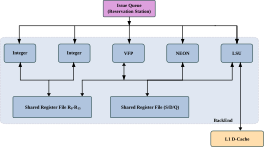
\includegraphics[width=7.8cm]{04_backend.pdf}
 \end{textblock*}
 \begin{textblock*}{7cm}(8.5cm,1.2cm)
  \justifying
  El Back-End utiliza dos Register Files independientes.
  \begin{itemize}[<+(1)->]\justifying
   \item El \textbf{Integer Register File} almacena los registros generales utilizados por las unidades enteras y por la LSU para calcular direcciones.
   \item El \textbf{Floating Point Register File} contiene los registros $S_{n}$, $D_{n}$ y $Q_{n}$ compartidos por VFP y NEON.
  \end{itemize}
 \end{textblock*}
 \begin{textblock*}{\textwidth}(0.3cm,5.8cm)
  \begin{itemize}[<+(1)->]\justifying
   \item Ambos pueden ser accedidos simultáneamente por diferentes unidades funcionales. (Puertos de lectura y escritura múltiples en ambos File Register)
   \item La LSU es el único bloque que interactúa con ambos Register Files y con la memoria.
  \end{itemize}
 \end{textblock*}
\end{frame}

\begin{frame}{Back-End: La Load/Store Unit}
 \begin{textblock*}{\textwidth}(0.4cm,1.2cm)
  \begin{tcolorbox}[enhanced jigsaw,rounded corners,drop fuzzy shadow=ShadowColor]
   \begin{itemize}[<+->]\justifying
    \item Todas las operaciones de lectura y escritura de memoria son realizadas exclusivamente por la \textbf{Load/Store Unit}.
    \item La LSU obtiene las direcciones desde el Integer Register File: $R_{0}-R_{15}$. Son los registros que trabajan como punteros a memoria en instrucciones Load / Store.
    \item En instrucciones VFP o NEON, la LSU transfiere datos entre la memoria y el VFP/SIMD Register File  $S_{n}$, $D_{n}$ y $Q_{n}$.
    \item Las unidades aritméticas Enteras, VFP y NEON nunca acceden directamente a la memoria; operan únicamente sobre datos previamente cargados en los registros correspondientes.
   \end{itemize}
  \end{tcolorbox}
 \end{textblock*}
\end{frame}

\begin{frame}{Back-End: Flujo de ejecución}
 \begin{textblock*}{\textwidth}(0.4cm,1.2cm)
  \begin{tcolorbox}[enhanced jigsaw,rounded corners,drop fuzzy shadow=ShadowColor]
   \begin{enumerate}[<+->]\justifying
    \item La lógica de Despacho selecciona una instrucción cuyos operandos ya están disponibles.
    \item La instrucción es enviada a la unidad funcional correspondiente.
    \item La unidad funcional lee los operandos desde el Register File adecuado.
    \item Finalizada la ejecución, el resultado es escrito nuevamente en el Register File, o en el caso de Instrucciones Load/Store es transferido desde o hacia la memoria mediante la LSU.
    \item Mientras una instrucción se ejecuta en una Unidad Funcional, otras instrucciones pueden ejecutarse simultáneamente en las restantes Unidades Funcionales (ILP).
   \end{enumerate}
  \end{tcolorbox}
 \end{textblock*}
\end{frame}

\begin{frame}{Back-End: Explotando el paralelismo}
 \begin{textblock*}{\textwidth}(0.4cm,1.2cm)
  \begin{tcolorbox}[enhanced jigsaw,rounded corners,drop fuzzy shadow=ShadowColor]
   \begin{itemize}[<+->]\justifying
    \item El objetivo del Back-End es mantener ocupadas simultáneamente la mayor cantidad posible de unidades funcionales.
    \item El rendimiento depende de la disponibilidad de instrucciones sin dependencias de datos, cuyos operandos estén listos para ser empleados en su ejecución (Esto se debe a la capacidad de Ejecución Fuera de Orden).
    \item En este marco, una unidad funcional ociosa equivale a un recurso desaprovechado y reduce el paralelismo a nivel de instrucción (ILP).
    \item En aplicaciones SIMD, la unidad NEON alcanza su máxima eficiencia cuando la LSU puede abastecerla continuamente desde la memoria.
   \end{itemize}
  \end{tcolorbox}
 \end{textblock*}
\end{frame}

\begin{frame}[fragile]{Recorrido de una instrucción por el Back-End}
 \begin{textblock*}{8cm}(0.3cm,1.2cm)
  \centering 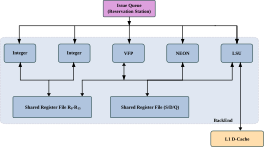
\includegraphics[width=7.8cm]{04_backend.pdf}
 \end{textblock*}
 \begin{textblock*}{7cm}(8.5cm,1.2cm)
  \begin{lstlisting}[basicstyle=\scriptsize,numbers=none, escapechar=\@]
VLD1.32  {Q0}, [R0]!
VLD1.32  {Q1}, [R1]!
VADD.F32   Q2, Q0, Q1
VST1.32  {Q2}, [R2]!
  \end{lstlisting}
  \begin{itemize}[<+(1)->] \justifying
   \item Las dos primeras instrucciones son accesos a memoria.
   \item La Issue Logic las envía a la \textbf{Load/Store Unit}.
   \item La LSU obtiene las direcciones desde el \textbf{Integer Register File}.
   \item Los datos son leídos desde la \textbf{L1 Data Cache}.
   \item Finalmente la LSU escribe los datos en los registros $Q_{0}$ y $Q_{1}$.
  \end{itemize}
 \end{textblock*}
\end{frame}

\begin{frame}[fragile]{Recorrido de una instrucción por el Back-End}
 \begin{textblock*}{8cm}(0.3cm,1.2cm)
  \centering 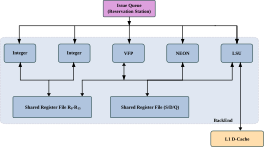
\includegraphics[width=7.8cm]{04_backend.pdf}
 \end{textblock*}
 \begin{textblock*}{7cm}(8.5cm,1.2cm)
  \begin{lstlisting}[basicstyle=\scriptsize,numbers=none, escapechar=\@]
VLD1.32  {Q0}, [R0]!
VLD1.32  {Q1}, [R1]!
VADD.F32   Q2, Q0, Q1
VST1.32  {Q2}, [R2]!
  \end{lstlisting}
  \begin{itemize}[<+(1)->] \justifying
   \item Una vez disponibles $Q_{0}$ y $Q_{1}$, la instrucción \texttt{\textbf{VADD.F32}} puede emitirse.
   \item La unidad \textbf{NEON} lee ambos operandos desde el banco de registros compartido.
   \item El resultado se escribe en $Q_{2}$.
   \item La instrucción \texttt{\textbf{VST1.32}} vuelve a ser ejecutada por la \textbf{Load/Store Unit}, que transfiere el contenido de $Q_{2}$ hacia la memoria.
  \end{itemize}
 \end{textblock*}
\end{frame}

\begin{frame}[fragile]{Ejemplo de ejecución en el Back-End}
 \begin{textblock*}{7.7cm}(0.3cm,1.2cm)
  \begin{lstlisting}[basicstyle=\scriptsize,numbers=none, escapechar=\@]
loop:

    VLD1.32   {Q0}, [R0]!
    VLD1.32   {Q1}, [R1]!

    ADD       R8, R8, #16
    SUBS      R9, R9, #1

    VADD.F32  Q2, Q0, Q1

    ADD       R10, R11, R12

    VMUL.F32  Q3, Q2, Q4

    STR       R10, [R7]

    VST1.32   {Q3}, [R2]!

    BNE       loop
  \end{lstlisting}
 \end{textblock*}
 \begin{textblock*}{7.2cm}(8.4cm,1.2cm)
  \justifying Esta secuencia permite ejecutar simultáneamente:
  \begin{itemize}[<+(1)->] \justifying
   \item instrucciones enteras;
   \item accesos a memoria;
   \item instrucciones SIMD NEON;
   \item dependencias de datos;
   \item oportunidades para explotar ILP.
  \end{itemize}
  \only<7>{
  Durante los siguientes slides seguiremos el recorrido de estas instrucciones sobre el Back-End del Cortex-A9.
  }
 \end{textblock*}
\end{frame}

\begin{frame}{Recorrido de las instrucciones sobre el Back-End (I)}
 \begin{textblock*}{8cm}(0.3cm,1.2cm)
  \centering 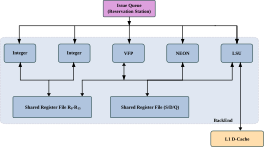
\includegraphics[width=7.8cm]{04_backend.pdf}
 \end{textblock*}
 \begin{textblock*}{7cm}(8.5cm,1.2cm)
  \begin{itemize}[<+(1)->]\justifying
   \item Las dos primeras instrucciones \texttt{\textbf{VLD1}} son enviadas a la \textbf{Load/Store Unit}.
   \item La LSU obtiene las direcciones desde los registros $R_{0}$ y $R_{1}$ del \textbf{Integer Register File}.
   \item Como hay una sola LSU esas dos instrucciones se ejecutan en serie.
   \item Los datos son transferidos desde la \textbf{L1 Data Cache} hacia el Register File de VFP y NEON: $S_{n}$, $D_{n}$ y $Q_{n}$.
  \end{itemize}
 \end{textblock*}
 \begin{textblock*}{\textwidth}(0.3cm,6.2cm)
  \begin{itemize}[<+(1)->]\justifying
   \item Mientras la LSU espera la respuesta de la memoria, las instrucciones
   \begin{center}
    \texttt{ADD} \hspace{3mm} y \hspace{3mm} \texttt{SUBS}
   \end{center}
   pueden ejecutarse en los \textbf{Integer Pipelines}.
\item \textit{El Back-End mantiene ocupadas tres de las unidades funcionales en forma simultánea.}
  \end{itemize}
 \end{textblock*}
\end{frame}

\begin{frame}{Recorrido de las instrucciones sobre el Back-End (II)}
 \begin{textblock*}{8cm}(0.3cm,1.2cm)
  \centering 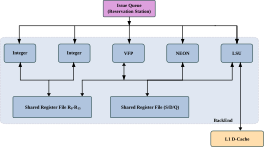
\includegraphics[width=7.8cm]{04_backend.pdf}
 \end{textblock*}
  \begin{textblock*}{7cm}(8.5cm,1.2cm)
   \begin{itemize}[<+(1)->]\justifying
    \item Una vez completadas ambas instrucciones \texttt{\textbf{VLD1}}, los registros $Q_{0}$ y $Q_{1}$ contienen operandos válidos.
    \item Ésto permite despachar:
    \begin{center}
    \texttt{\textbf{VADD.F32 Q2,Q0,Q1}}
    \end{center}
    hacia la unidad \textbf{NEON}.
    \item La instrucción
    \begin{center}
    \texttt{\textbf{VMUL.F32 Q3,Q2,Q4}}
    \end{center}
    debe esperar la finalización de \texttt{\textbf{VADD}}.
   \end{itemize}
  \end{textblock*}
 \begin{textblock*}{\textwidth}(0.3cm,6.2cm)
  \begin{itemize}[<+(1)->]\justifying
  \item Pero la instrucción
  \begin{center} \textbf{\texttt{ADD  R10, R11, R1}},\end{center}
  puede despacharse a una Unidad de Ejecución de Enteros, ya que ya deben haberse liberado de las dos instrucciones enteras anteriores.
  \end{itemize}
 \end{textblock*}
\end{frame}

\begin{frame}{Recorrido de las instrucciones sobre el Back-End (III)}
 \begin{textblock*}{8cm}(0.3cm,1.2cm)
  \centering 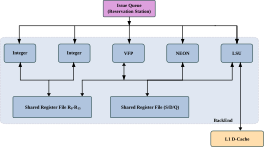
\includegraphics[width=7.8cm]{04_backend.pdf}
 \end{textblock*}
 \begin{textblock*}{7cm}(8.5cm,1.2cm)
  \begin{itemize}[<+(1)->]\justifying
   \item La instrucción
   \begin{center} \textbf{\texttt{STR  R10, [R7]}},\end{center}
   puede despacharse a la LSU, ya que se terminaron de ejecutar las dos instrucciones \textbf{\texttt{VLD1.32 }} anteriores.
   \item Finalmente la instrucción
   \begin{center}
   \textbf{\texttt{VST1.32 \{Q3\},[R2]!}}
   \end{center}
   es ejecutada por la \textbf{Load/Store Unit}, que transfiere el resultado hacia la memoria.
  \end{itemize}
 \end{textblock*}
 \begin{textblock*}{\textwidth}(0.3cm,6.2cm)
 \end{textblock*}
\end{frame}

\begin{frame}{¿Dónde aparece el Instruction-Level Parallelism?}
 \begin{textblock*}{\textwidth}(0.4cm,1.2cm)
  \begin{tcolorbox}[enhanced jigsaw,rounded corners,drop fuzzy shadow=ShadowColor]
   \begin{itemize}[<+->]\justifying
    \item Las instrucciones \texttt{\textbf{VADD}} y \textbf{\texttt{VMUL}} deben esperar a que estén disponibles sus operandos, generando dependencias de tipo \textbf{RAW}.
    \item Sin embargo, las instrucciones enteras \texttt{\textbf{ADD}} y \texttt{\textbf{SUBS}} son independientes y pueden ejecutarse mientras la LSU espera la respuesta de la memoria.
    \item El procesador aprovecha estas oportunidades para mantener ocupadas simultáneamente distintas unidades funcionales.
    \item La ejecución fuera de orden no modifica el resultado del programa; únicamente altera el instante en que cada instrucción es ejecutada.
    \item Riesgo WAW: las instrucciones \texttt{\textbf{STR}} y \textbf{\texttt{ADD}} se despachan en el mismo ciclo y escriben sobre el registro $R_{10}$. El Cortex-A9 permite ejecutar fuera de orden evitando este riesgo. Sin embargo, la escritura en memoria consume dos ciclos de cómputo frente a un solo ciclo de la suma, de modo que termina antes la instrucción mas antigua y naturalmente el commit a $R_{10}$ ocurre en orden.
   \end{itemize}
  \end{tcolorbox}
 \end{textblock*}
\end{frame}


\begin{frame}{Subsistema de memoria del Cortex-A9}
 \begin{textblock*}{8cm}(0.3cm,1.2cm)
  \centering 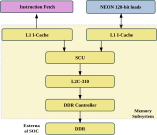
\includegraphics[width=7.8cm]{05_memory.pdf}
 \end{textblock*}
 \begin{textblock*}{7cm}(8.5cm,1.2cm)
 \justifying El subsistema de memoria abastece tanto el flujo de instrucciones para el Front End, como también los datos requeridos por el Back-End.
  \begin{itemize}[<+(1)->]
   \item Caché L1 separada para instrucciones y datos (arquitectura Harvard modificada).
   \item Caché L2 unificada y compartida por ambos núcleos del Cortex-A9 MPCore.
   \item La \textbf{SCU} mantiene la coherencia entre las cachés L1 de ambos núcleos.
   \item La memoria DDR constituye el último nivel de la jerarquía.
  \end{itemize}
 \end{textblock*}
\end{frame}

\begin{frame}{Split Cache: instrucciones y datos}
 \begin{textblock*}{8cm}(0.3cm,1.2cm)
  \centering 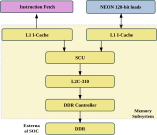
\includegraphics[width=7.8cm]{05_memory.pdf}
 \end{textblock*}
 \begin{textblock*}{7cm}(8.5cm,1.2cm)
  \justifying
  La separación entre la caché de instrucciones y la caché de datos permite realizar accesos simultáneos.
  \begin{itemize}[<+(1)->]\justifying
   \item El Front-End obtiene continuamente instrucciones desde la L1 I-Cache.
   \item En paralelo, la LSU accede a la L1 D-Cache para cargar y almacenar datos.
   \item Ambos accesos se realizan sin competir por el mismo recurso físico.
   \item Esta organización resulta especialmente importante en aplicaciones SIMD con un elevado tráfico de memoria.
  \end{itemize}
 \end{textblock*}
\end{frame}

\begin{frame}{El subsistema de memoria y el rendimiento de NEON}
 \begin{textblock*}{\textwidth}(0.4cm,1.2cm)
  \begin{tcolorbox}[enhanced jigsaw,rounded corners,drop fuzzy shadow=ShadowColor]
   \begin{itemize}[<+->]\justifying
    \item La unidad \textbf{NEON} ejecuta operaciones únicamente sobre datos residentes en el banco de registros $S_{n}$, $D_{n}$ y $Q_{n}$.
    \item Los datos deben ser transferidos previamente desde memoria mediante la \textbf{Load/Store Unit}.
    \item Si la \textbf{LSU} o la jerarquía de memoria no suministran datos con suficiente velocidad, la unidad \textbf{NEON} permanece ociosa.
    \item En aplicaciones \textbf{SIMD}, el rendimiento depende tanto de la capacidad de cálculo como del ancho de banda efectivo del subsistema de memoria.
   \end{itemize}
   \vspace {0.3cm}
  \only<5->{Duplicar la potencia de cálculo de \textbf{NEON} no mejora el rendimiento si los datos llegan desde memoria a la misma velocidad. En aplicaciones SIMD es frecuente que el cuello de botella no sea la unidad de ejecución, sino el subsistema de memoria.}
  \end{tcolorbox}
 \end{textblock*}
\end{frame}

\begin{frame}{Organización funcional de la unidad NEON}
 \begin{textblock*}{.22\textwidth}(0.3cm,1.2cm)
  \centering 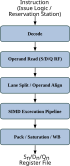
\includegraphics[width=.9\textwidth]{06_neon_pipeline_01.pdf}
 \end{textblock*}
 \begin{textblock*}{.78\textwidth}(.24\textwidth,1.2cm)
  \justifying \textbf{NEON} es la unidad funcional especializada en procesamiento SIMD.
  \begin{itemize}[<+(1)->]\justifying
   \item Recibe instrucciones desde la \textbf{Issue Logic} del Back-End.
   \item Decode: identifica el tipo de operación, y determina el tamaño de cada elemento (8, 16, 32, \SI{64}{\bit}).
   \item Obtiene uno o dos operandos desde el Register File $S_{n}$, $D_{n}$ y $Q_{n}$.
   \item Lane Split/Align: separa los operandos en lanes, selecciona el formato, y realiza extensiones de signo o cero cuando corresponde.
   \item Ejecuta operaciones sobre múltiples elementos en paralelo (suma, multiplicación, lógica, comparaciones, etc.).
   \item Pack / Saturation / Write Back: recompone el registro, aplica saturación cuando la instrucción lo requiere, y escribe los resultados nuevamente en el Register File Compartido.
  \end{itemize}
  \only<8>{
  Internamente, NEON está organizada como un pipeline compuesto por varias etapas especializadas.
  }
 \end{textblock*}
\end{frame}

\begin{frame}{Registros NEON y concepto de \textit{lanes}}
 \begin{textblock*}{8cm}(0.3cm,1.2cm)
  \centering
  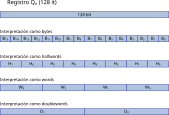
\includegraphics[width=7.8cm]{07_neon_lanes.pdf}
 \end{textblock*}
 \begin{textblock*}{7cm}(8.5cm,1.2cm)
 \justifying
 Los registros $Q_{n}$ poseen un ancho fijo de \SI{128}{\bit}. Sin embargo, la unidad NEON no interpreta este registro como un único operando de \SI{128}{\bit}.
 \begin{itemize}[<+(1)->] \justifying
  \item Cada registro se divide en varios elementos llamados \textbf{lanes}.
  \item El tamaño de cada \textit{lane} depende del tipo de dato especificado por la instrucción.
  \item Todos los \textit{lanes} ejecutan simultáneamente la misma operación.
  \item Este modelo constituye la esencia del procesamiento \textbf{SIMD}.
 \end{itemize}
 \end{textblock*}
\end{frame}


\begin{frame}{Pipeline funcional de la unidad NEON}
 \begin{textblock*}{.22\textwidth}(0.3cm,1.2cm)
  \centering 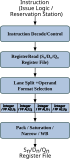
\includegraphics[width=.9\textwidth]{08_neon_pipeline.pdf}
 \end{textblock*}
 \begin{textblock*}{.76\textwidth}(.26\textwidth,1.2cm)
  \justifying Una vez despachada por la Reservation Station \textbf{Issue}, la instrucción atraviesa varias etapas internas antes de completar su ejecución.
  \begin{itemize}[<+(1)->]\justifying
   \item Lectura de operandos desde el Register File $S_{n}/D_{n}/Q_{n}$.
   \item Separación de los operandos en \textit{lanes} y adaptación al formato de datos solicitado.
   \item Ejecución simultánea de la operación sobre todos los \textit{lanes}.
   \item Reensamblado del resultado y escritura en el banco de registros.
  \end{itemize}
  \only<6>{
  Una nueva instrucción puede ingresar al pipeline antes de que la anterior haya finalizado, incrementando el throughput de la unidad.
 }
 \end{textblock*}
\end{frame}

\begin{frame}{Interpretación de las tablas de tiempos del TRM}
 \begin{textblock*}{\textwidth}(0.4cm,1.2cm)
  \justifying En el documento de ARM llamado ``Cortex™ -A9 NEON™ Media Processing Engine. Revision: r4p0. Technical Reference Manual'', el capítulo 3 está dedicado al Timing de las Instrucciones. Allí encontraremos Tablas como la siguiente abarcando todo el set deinstrucciones VFP / NEON.
  \begin{center}
   \small
   \begin{tabular}{|c|c|c|c|c|}
    \hline
    Instruction & Cycles & Source & Result & Write Back \\
    \hline
    VADD.F32 & 1 & -,2,2 & 5 & 6 \\
    VMUL.F32 & 1 & -,2,2 & 6 & 7 \\
    \hline
   \end{tabular}
  \end{center}
  \begin{itemize}[<+(1)->]\justifying
   \item \textbf{Cycles}: Cantidad de ciclos durante los cuales la instrucción ocupa la etapa de Envío (Issue) de su unidad funcional. Determina el throughput máximo de esa unidad.
   \item \textbf{Source}: Indica el ciclo interno del Pipeline NEON en el que cada operando debe estar disponible. Si el dato aún no está disponible (registro o forwarding), la instrucción no puede continuar su ejecución.
   \item \textbf{Result}: ciclo en el que el resultado ya puede ser utilizado mediante forwarding.
   \item \textbf{Write Back}: ciclo en el que el resultado se almacena en el Register File.
  \end{itemize}
 \end{textblock*}
\end{frame}

\begin{frame}{Pipeline NEON: Latencia y Throughput}
 \begin{textblock*}{8.2cm}(0.3cm,1.2cm)
  \centering
  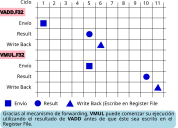
\includegraphics[width=7.6cm]{09_neon_timeline.pdf}
  \vspace{-0.4cm}
  \only<5> {
   \begin{tcolorbox}[enhanced jigsaw,rounded corners,drop fuzzy shadow=ShadowColor]
    \justifying Mantener el pipeline continuamente ocupado constituye uno de los principales objetivos de la ejecución fuera de orden.
   \end{tcolorbox}
  }
 \end{textblock*}
 \begin{textblock*}{7cm}(8.5cm,1.2cm)
  \justifying
  Una instrucción SIMD permanece varios ciclos dentro del pipeline antes de finalizar su ejecución.
  \begin{itemize}[<+(1)->]\justifying
   \item El \textbf{latency} es el tiempo transcurrido desde que una instrucción ingresa al pipeline hasta que su resultado queda disponible.
   \item El \textbf{throughput} indica la velocidad con la que el pipeline puede aceptar nuevas instrucciones.
   \item Un pipeline puede tener un latency de varios ciclos y, al mismo tiempo, admitir el ingreso de una nueva instrucción en cada ciclo de reloj.
  \end{itemize}
 \end{textblock*}
\end{frame}


\begin{frame}[fragile]{Ejecución del bucle sobre el Back-End}
 \begin{textblock*}{4.2cm}(0.3cm,1.2cm)
  \scriptsize
  \begin{lstlisting}[basicstyle=\scriptsize,numbers=none, escapechar=\@]
loop:
    VLD1.32  {Q0}, [R0]!
    VLD1.32  {Q1}, [R1]!

    ADD      R8, R8, #16
    SUBS     R9, R9, #1

    VADD.F32 Q2, Q0, Q1
    ADD      R10,R11,R12
    VMUL.F32 Q3, Q2, Q4

    STR      R10,[R7]
    VST1.32  {Q3},[R2]!
    BNE      loop
  \end{lstlisting}
 \end{textblock*}
 \begin{textblock*}{11cm}(4.3cm,1.2cm)
  \only<2->{\centering 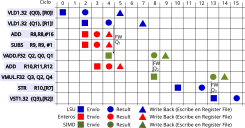
\includegraphics[width=.85\textwidth]{10_full_timeline.pdf}}
 \end{textblock*}
 \begin{textblock*}{\textwidth}(0.4cm,6.1cm)
 \only<3->{
  \begin{tcolorbox}[enhanced jigsaw,rounded corners,drop fuzzy shadow=ShadowColor]
   \begin{itemize}[<+(2)->]\scriptsize\justifying
    \item Las dos instrucciones \texttt{VLD1} generan un cuello de botella inicial al compartir la única \textbf{Load/Store Unit}.
    \item Mientras la LSU accede a memoria, los dos \textbf{Integer Pipelines} ejecutan instrucciones independientes.
    \item La instrucción \texttt{VADD} debe esperar la disponibilidad de los operandos cargados por la LSU.
    \item El resultado de \texttt{VADD} es consumido por \texttt{VMUL} mediante \textbf{forwarding}, sin esperar el \textit{Write Back}.
    \item Finalmente, la LSU vuelve a intervenir para almacenar el resultado mediante \texttt{VST1}.
   \end{itemize}
  \end{tcolorbox}
  }
 \end{textblock*}
\end{frame}

\section{Set de instrucciones}
\subsection{Sintaxis}

\begin{frame}[fragile]{Sintaxis de instrucciones NEON}
 \begin{textblock*}{\textwidth}(0.4cm,1.2cm)
 \only<1->{
  \begin{tcolorbox}[enhanced jigsaw,rounded corners, drop fuzzy shadow=ShadowColor]
  \begin{itemize}[<+(1)->]\justifying
   \item Una misma instrucción puede operar sobre diferentes tipos de datos.
   \item El tipo de dato se especifica como sufijo de la instrucción.
   \item La cantidad de datos (lanes) empaquetados, depende del tipo de dato y de los registros empleados.
   \item Hemos visto ejemplos de instrucciones que muestran esta definición.
   \item Sin embargo hay casos en los que los tamaños de registro no son homogéneos
  \end{itemize}
  \end{tcolorbox}
  }
 \end{textblock*}
 \begin{textblock*}{\textwidth}(0.4cm,5.4cm)
  \begin{onlyenv}<7>
   \begin{lstlisting}[basicstyle=\scriptsize,numbers=none, escapechar=\@]
VMULL.S16 Q2, D8, D9    // Vector MULtiply Long
                        // Q2[3]=D8[3]*D9[3], Q2[2]=D8[2]*D9[2]
                        // Q2[1]=D8[1]*D9[1], Q2[0]=D8[0]*D9[0]
   \end{lstlisting}
  \end{onlyenv}
 \end{textblock*}
\end{frame}

\begin{frame}[fragile]{Sintaxis de instrucciones NEON}
 \begin{textblock*}{\textwidth}(0.4cm,1.2cm) 
  Formato General:
  \begin{lstlisting}[basicstyle=\scriptsize,numbers=none, escapechar=\@]
  V{<mod>}<op>{<shape>}{<cond>}{.<dt>} <dest1>{, <dest2>}, <src1>{, <src2>}
  \end{lstlisting}
 \end{textblock*}
 \begin{textblock*}{.94\textwidth}(1cm,2.9cm) 
  \begin{itemize} \justifying
   \item [\textit{mod}] Modificador: \textbf{Q} Saturado, \textbf{H} Halfing, \textbf{D} Doubling, \textbf{R} Redondeado
   \item [\textit{op}] Operación: Es la operación en sí (por ejemplo ADD, MUL, etc)
   \item [\textit{shape}] Modificador: \textbf{L} Long, \textbf{W} Wide, o \textbf{N} Narrow.
   \item [\textit{cond}] Condition: Se utiliza como ya sabemos con la instrucción IT.
   \item [\textit{dt}] Data Type
   \item [\textit{dest\textsubscript{n}}] Registro o registros destino
   \item [\textit{src\textsubscript{n}}] Registro o registros fuente
  \end{itemize}
 \end{textblock*}
\end{frame}

\begin{frame}{Modificadores de Instrucción}
 \begin{scriptsize}
  \begin{center}
   \begin{textblock*}{\textwidth}(0.4cm,1.2cm)
    \begin{tikzpicture}
     \node (tbl) { 
      \rowcolors[]{1}{}{gray!5}
      \begin{tabularx}{.98\textwidth}{p{.05\textwidth} p{.12\textwidth} p{.25\textwidth} p{.45\textwidth} }
       \textbf{\color{white} Modif.} & \textbf{\color{white} Acción} & \textbf{ \color{white} Ejemplo} & \textbf{ \color{white} Descripción}\\
       Nada & Op. Básica & VADD.I16 Q0, Q1, Q2 & Resultado sin modificación\\
       Q & Saturation & VQADD.S16 D0, D2, D3 & Si el resultado satura el rango, queda en el máximo o mínimo valor según corresponda.\\
       H & Halved & VHADD.S16 Q0, Q1, Q4 & Cada operando se desplaza un lugar a la derecha antes de su uso (división por dos con truncado). En el ejemplo se calcula un promedio con truncado\\
       D & Doubled & VQDMULL.S16 Q0, D1, D3 & Se duplica el resultado (D), y si el valor excede el rango del operando destino, se satura (Q): $Q_{0}= 2*(D_{1}*D_{3})$. Especialmente útil cuando se trabaja en punto fijo formato Q15 (caso muy frecuente en DSP), en donde se requiere adaptar el rango del resultado en los productos. La segunda L del opcode indica que el resultado ocupa elementos del doble de tamaño que los operandos. Dedicaremos los dos slides siguientes esta instrucción en el marco del formato Q15\\
       R & Rounded & VRSUBHN.I16 D0, Q1, Q3 & Redondea la división por dos del resultado (H), para corregir el error de truncado. Equivale a sumar 0.5 antes de truncar. La N implica que el resultado ocupa un elemento de la mitad del tamaño de los operandos.\\
       \end{tabularx}
     };
     \begin{pgfonlayer}{background}
      \draw[rounded corners,top color=red,bottom color=black,draw=white] ($(tbl.north west)+(0.14,0)$) rectangle ($(tbl.north east)-(0.13,0.45)$);
      \draw[rounded corners,top color=white,bottom color=black, middle color=red,draw=blue!20] ($(tbl.south west)+(0.12,0.5)$) rectangle ($(tbl.south east)-(0.12,0)$);
      \draw[top color=blue!1,bottom color=blue!20,draw=white] ($(tbl.north east)-(0.13,0.6)$) rectangle ($(tbl.south west)+(0.13,0.2)$);
     \end{pgfonlayer}
    \end{tikzpicture}
   \end{textblock*} 
  \end{center}
 \end{scriptsize}
\end{frame}

\begin{frame}{Representación en Punto Fijo Q15}
 \begin{textblock*}{\textwidth}(0.4cm,1.2cm)
%   \begin{tcolorbox}[enhanced jigsaw,rounded corners,drop fuzzy shadow=ShadowColor]
   \begin{itemize}[<+->]\justifying
    \item En procesamiento digital de señales (DSP) es frecuente representar números reales mediante \textbf{punto fijo} para evitar el costo del hardware de punto flotante.
    \item El formato \textbf{Q15} utiliza un entero con signo de \SI{16}{\bit} interpretando que el punto binario se encuentra inmediatamente antes del bit de signo.
    \item El rango representable es aproximadamente: $-1.0 \le x < 1.0$
    \item La conversión entre el valor entero almacenado y el valor real es:
    $x=\frac{\text{entero}}{2^{15}}$
    \item Algunos ejemplos son:
    \[
     \begin{array}{c|c}
      \textbf{Entero} & \textbf{Valor Q15} \\
      \hline
      32767 & 0.99997 \\
      16384 & 0.5 \\
      8192  & 0.25 \\
      0     & 0.0 \\
      -32768 & -1.0
     \end{array}
    \]
   \end{itemize}
%   \end{tcolorbox}
 \end{textblock*}
\end{frame}

\begin{frame}{¿Por qué existe la instrucción VQDMULL?}
 \begin{textblock*}{\textwidth}(0.4cm,1.2cm)
  \begin{tcolorbox}[enhanced jigsaw,rounded corners,drop fuzzy shadow=ShadowColor]
   \begin{itemize}[<+->]\justifying
    \item Al multiplicar dos valores Q15 se obtiene un resultado de \SI{32}{\bit}.\\
    $ Q15 \times Q15 \longrightarrow Q30$
    \item El resultado queda escalado \SI{1}{\bit} por debajo del formato Q31 habitualmente utilizado para acumulación.
    \item La instrucción \texttt{VQDMULL.S16 Q0, D1, D3} realiza automáticamente: $\boxed{2 \times (A \times B)}$,equivalente a un desplazamiento a la izquierda de un bit. $A$ y$B$ representan cada lane de $D_{1}$ y $D_{3}$
    \item De este modo: $Q30 \xrightarrow{\times 2} Q31$,  manteniendo la normalización de los datos.
    \item La operación incorpora además \textbf{saturación}, evitando overflow durante el desplazamiento.
   \end{itemize}
  \end{tcolorbox}
 \end{textblock*}
\end{frame}

\begin{frame}{VRSUBHN: retorno al formato original}
 \begin{textblock*}{\textwidth}(0.4cm,1.2cm)
  \begin{itemize}[<+->]\justifying
   \item Durante el procesamiento DSP es habitual realizar los cálculos con mayor precisión que la de los datos originales.
   \item Luego de una secuencia de multiplicaciones y acumulaciones en \SI{32}{\bit}, es necesario volver al formato Q15 para almacenar o continuar el procesamiento.
   \item La instrucción \texttt{VRSUBHN} (\textbf{Vector Rounding Subtract High Narrow}) realiza simultáneamente:
   \begin{itemize}
    \item una resta entre operandos de precisión extendida;
    \item un redondeo del resultado;
    \item la extracción de la mitad alta (\textit{High});
    \item la reducción del ancho (\textit{Narrow}) al tamaño original.
   \end{itemize}
   \item Conceptualmente:
$ \boxed{
32\ \text{bits}
\;\longrightarrow\;
16\ \text{bits}
}
$
   preservando la mayor precisión posible gracias al redondeo previo.
   \item En aplicaciones DSP suele utilizarse como etapa final luego de operaciones como \texttt{VMULL} o \texttt{VQDMULL}, permitiendo regresar al formato Q15 con el menor error de cuantización posible.
  \end{itemize}
 \end{textblock*}
\end{frame}

\begin{frame}[fragile]{Formas de Instrucción}
 \begin{textblock*}{.48\textwidth}(0.4cm,1.2cm)
  \begin{onlyenv}<1->
   \begin{tcolorbox}[enhanced jigsaw,rounded corners, drop fuzzy shadow=ShadowColor]
    \textbf{No especificado}:\\ Operandos y resultados son del mismo tamaño.\\
    Ej:
    \begin{lstlisting}[basicstyle=\scriptsize,numbers=none]
VADD.I16 Q0, Q1, Q2
    \end{lstlisting}
   \end{tcolorbox}
  \end{onlyenv} 
 \end{textblock*}
 \begin{textblock*}{.48\textwidth}(0.4cm+.5\textwidth,1.2cm)
  \begin{onlyenv}<2->
   \begin{tcolorbox}[enhanced jigsaw,rounded corners, drop fuzzy shadow=ShadowColor]
    \textbf{Long-L}:\\ Operandos del mismo tamaño, y resultados del doble de tamaño.\\
    Ej:
    \begin{lstlisting}[basicstyle=\scriptsize,numbers=none]
VADDL.S16 Q0, D2, D3
    \end{lstlisting}
   \end{tcolorbox}
  \end{onlyenv} 
 \end{textblock*}
 \begin{textblock*}{.48\textwidth}(0.4cm,4.9cm)
  \begin{onlyenv}<3->
   \begin{tcolorbox}[enhanced jigsaw,rounded corners, drop fuzzy shadow=ShadowColor]
    \textbf{Narrow-N}:\\ Operandos del mismo tamaño, y resultados de la mitad de tamaño.\\
    Ej:
    \begin{lstlisting}[basicstyle=\scriptsize,numbers=none]
VADDL.S16 D0, Q2, Q3
    \end{lstlisting}
   \end{tcolorbox}
  \end{onlyenv} 
 \end{textblock*}
 \begin{textblock*}{.48\textwidth}(0.4cm+.5\textwidth,4.9cm)
  \begin{onlyenv}<4->
   \begin{tcolorbox}[enhanced jigsaw,rounded corners, drop fuzzy shadow=ShadowColor]
    \textbf{Wide-W}: \\El tamaño del resultado y 1er. operando es el doble del 2do. operando.\\
    Ej:
    \begin{lstlisting}[basicstyle=\scriptsize,numbers=none]
VADDW.I16 Q0, Q1, D4
    \end{lstlisting}
   \end{tcolorbox}
  \end{onlyenv} 
 \end{textblock*} 
\end{frame}

\begin{frame}{NEON Long Instruction}
 \begin{textblock*}{\textwidth}(0.4cm,1.1cm)
  \begin{center} 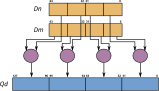
\includegraphics[width=.8\textwidth]{Neon-Long.pdf}\end{center}
 \end{textblock*} 
\end{frame}

\begin{frame}{NEON Wide Instruction}
 \begin{textblock*}{\textwidth}(0.4cm,1.1cm)
  \begin{center} 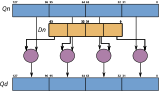
\includegraphics[width=.8\textwidth]{Neon-Wide.pdf}\end{center}
 \end{textblock*} 
\end{frame}

\begin{frame}{NEON Narrow Instruction}
 \begin{textblock*}{\textwidth}(0.4cm,1.1cm)
  \begin{center} 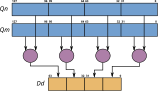
\includegraphics[width=.8\textwidth]{Neon-Narrow.pdf}\end{center}
 \end{textblock*} 
\end{frame}

\begin{frame}{Empaquetado y desempaquetado de datos}
 \begin{textblock*}{\textwidth}(0.4cm,1.1cm)
  \begin{itemize}[<+(1)->]\justifying
   \item NEON trabaja con datos empaquetados en un registro para procesarlos en una única instrucción.
   \item La preparación de esos operandos, lo mismo que la extracción de los resultados empaquetados no siempre pueden llevarse a cabo con instrucciones NEON
   \item Existen para ayudar a esta tarea algunas instrucciones ARMv7 comunes para manipular los datos pre y post procesamiento NEON.
  \end{itemize}
 \end{textblock*}
 \begin{textblock*}{\textwidth}(0.4cm,4.0cm)
  \begin{onlyenv}<5->
   \begin{center}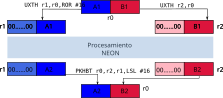
\includegraphics[width=0.65\textwidth]{Neon-Pack-Unpack.pdf}\end{center}
  \end{onlyenv}
 \end{textblock*} 
\end{frame}

\begin{frame}[fragile]{Empaquetado y desempaquetado de datos}
 \begin{textblock*}{\textwidth}(0.4cm,1.1cm)
  \begin{tcolorbox}[enhanced jigsaw,rounded corners, drop fuzzy shadow=ShadowColor]
    \textbf{UXTH}\\
Extensión de ceros a un halfword. Extiende un valor de \SI{16}{\bit} a \SI{32}{\bit}.
\begin{lstlisting}[basicstyle=\scriptsize,numbers=none]
UXTH{cond} {Rd}, Rm {,rotation}
\end{lstlisting}
\texttt{rotation} es la cantidad de bits que se rota a derecha \texttt{Rm} antes de enviar su halfword menos significativa al Registro destino (\texttt{Rd}). Puede ser \texttt{\#ROR 8, \#ROR 16, \#ROR 24}
  \end{tcolorbox}
 \end{textblock*} 
\end{frame}

\begin{frame}[fragile]{Empaquetado y desempaquetado de datos}
 \begin{textblock*}{\textwidth}(0.4cm,1.1cm)
  \begin{tcolorbox}[enhanced jigsaw,rounded corners, drop fuzzy shadow=ShadowColor]
    \textbf{PKHBT} y \textbf{PKHTB}\\
Instrucciones de empaquetado de Halfword. Combinan las halfwords de un registro con una halfword de otro regitro. El segundo de los registros origen puede ser desplazado n bits a derecha o izquierda antes de la extracción del dato.
\begin{lstlisting}[basicstyle=\scriptsize,numbers=none]
PKHBT{cond} {Rd}, Rn, Rm{, LSL #leftshift}
PKHTB{cond} {Rd}, Rn, Rm{, ASR #rightshift}
\end{lstlisting}
\textbf{PKHBT} Combina Rn[15:0] con Rm[31:16] previamente desplazado.\\
\textbf{PKHTB} Combina Rn[31:16] con Rm[15:0] previamente desplazado.\\
$ 0 \leq leftshift \leq 31, y 1 \leq rightshift \leq 32$
  \end{tcolorbox}
 \end{textblock*} 
\end{frame}

\begin{frame}[fragile]{Alineación de datos}
 \begin{textblock*}{\textwidth}(0.4cm,1.1cm)
  \begin{itemize}[<+(1)->]\justifying
   \item Si bien hay un soporte a la alineación de datos a nivel de arquitectura ARMv7, además se incluye en las instrucciones NEON que operan con memoria, la capacidad de especificar la alineación de datos deseada.
   \item De mas está decir que ésta especificación debe ser consistente con el tipo de operandos de la instrucción.
   \item Si la dirección de memoria no resulta consistente con el alineamiento especificado, se genera una Data Abort exception.
  \end{itemize}
 \end{textblock*}
 \begin{textblock*}{\textwidth}(0.8cm,4.7cm)
  \begin{onlyenv}<5->
   \begin{lstlisting}[basicstyle=\scriptsize,numbers=none]
VLD1.8 {D0},         [R1:64]       // D0[0]=[R1], D0[1]=[R1+1]...D0[7]=[R1+7]
VLD1.8 {D0,D1},      [R4:128]!     // ! : Finalizada, R4 se incrementa.
VLD1.8 {D0,D1,D2,D3},[R7:256], R2  // R2 offset que se suma a R7.
   \end{lstlisting}
  \end{onlyenv} 
 \end{textblock*}
 \begin{textblock*}{\textwidth}(0.4cm,6.2cm)
  \begin{itemize}[<+(2)->]\justifying
   \item La alineación se expresa en la instrucción como \texttt{<Reg>:<align>}.
   \item En el manual de instrucciones ARMv7 la alineación se expresa como un número precedido de '@'. No es necesaria en el código fuente.
  \end{itemize}
 \end{textblock*} 
\end{frame}


\subsection{Aritmética en algoritmos DSP}
\begin{frame}{Acumulación de resultados sobre un registro}
 \begin{textblock*}{\textwidth}(0.4cm,1.2cm)
  \begin{itemize}[<+(1)->]\justifying
   \item A medida que acumulamos resultados en un registro, llegamos inexorablemente al punto en el que el rango del resultado excede la capacidad de bits del registro de acumulación.
   \item En este punto los procesadores convencionales indican la situación mediante un flag de overflow, y en el operando destino se almacena el valor de \textbf{desborde}.
   \item La aplicación chequea dentro del lazo de cálculo este flag y de acuerdo a su estado decide si sigue la acumulación.
   \item El costo de esta práctica de programación es tiempo de ejecución para analizar como tratar cada resultado parcial.
  \end{itemize}
 \end{textblock*} 
\end{frame}

\begin{frame}[t,fragile]{Manejo de los desbordes}
 \begin{textblock*}{\textwidth}(0.4cm,1.3cm)
  \begin{onlyenv}<2->
   \begin{tcolorbox}[enhanced jigsaw,rounded corners, drop fuzzy shadow=ShadowColor]
    Resumen del comportamiento planteado en el slide anterior: Al llegar al extremo superior del rango, los procesadores convencionales realizan una operación de que se denomina wraparound, (reset del contador al valor inicial y activar flag de overflow). Si se decrementa un registro, por debajo de cero se pasa al valor máximo y se sigue desde allí.\\ Esto se conoce como \textit{Aritmética de Desborde}.\\
    El costo es comprobar en cada ciclo de un lazo el valor del flag para decidir si se continúa en el lazo o no. 
   \end{tcolorbox}
  \end{onlyenv}
 \end{textblock*} 
 \begin{textblock*}{\textwidth}(0.4cm,6.0cm)
  \begin{onlyenv}<3->
   \begin{tcolorbox}[enhanced jigsaw,rounded corners, drop fuzzy shadow=ShadowColor]
    Cuando se implementa \textit{Aritmética Saturada}, al producirse una condición fuera de rango el operando destino mantiene el máximo o mínimo valor del rango (dependiendo si la condición se ha producido por exceso o por defecto).
   \end{tcolorbox}
  \end{onlyenv}
 \end{textblock*} 
\end{frame}

\begin{frame}{Aritmética Saturada}
 \begin{textblock*}{\textwidth}(0.4cm,1.2cm)
  \begin{onlyenv}<2->
   \begin{table}[h]
    \rowcolors{1}{blue4}{blue4}
    \begin{tabular}{|c|c|c|c|c|} \hline
     \multicolumn{1}{|c|}{} & \multicolumn{2}{|c|}{\color{white} Límite Inferior} & \multicolumn{2}{c|}{\color{white}Límite Superior}\\ \cline{2-5}\cline{2-5}
     \multicolumn{1}{|c|}{\multirow{-2}{*}{\color{white}Tipo de Dato}} & \multicolumn{1}{|c|}{\color{white}Hexadecimal} & \color{white}Decimal & \color{white}Hexadecimal & \color{white}Decimal\\ \hline
     \rowcolor{gray!20} byte signado & 0x80 & -128 & 0x7F & 127 \\ \hline
     \rowcolor{gray!80} word signada & 0x8000 & -32768 & 0x7FFF & 32767 \\ \hline
    \end{tabular}
    \begin{center} Aritmética Saturada Signada \end{center}
   \end{table}
  \end{onlyenv}
 \end{textblock*} 
 \begin{textblock*}{\textwidth}(0.4cm,4.4cm)
  \begin{onlyenv}<3->
   \begin{table}[h]
    \rowcolors{1}{blue4}{blue4}
    \begin{tabular}{|c|c|c|c|c|} \hline
     \multicolumn{1}{|c|}{} & \multicolumn{2}{|c|}{\color{white} Límite Inferior} & \multicolumn{2}{c|}{\color{white}Límite Superior}\\ \cline{2-5}\cline{2-5}
     \multicolumn{1}{|c|}{\multirow{-2}{*}{\color{white}Tipo de Dato}} & \multicolumn{1}{|c|}{\color{white}Hexadecimal} & \color{white}Decimal & \color{white}Hexadecimal & \color{white}Decimal\\ \hline
     \rowcolor{gray!20} byte no signado & 0x00 & 0 & 0xFF & 255 \\ \hline
     \rowcolor{gray!80} word no signada & 0x0000 & 0 & 0xFFFF & 65535 \\ \hline
    \end{tabular}
    \begin{center} Aritmética Saturada No Signada \end{center}
   \end{table}
  \end{onlyenv}
 \end{textblock*} 
\end{frame}

\begin{frame}{Aritmética Saturada vs. Aritmética de Desborde}
 \begin{textblock*}{\textwidth}(0.4cm,1.2cm)
  \begin{itemize}[<+(1)->] \justifying \parskip 0.2cm
   \item Consideremos la siguiente suma empaquetada de 8 bytes.
  \end{itemize}
 \end{textblock*} 
 \begin{textblock*}{\textwidth}(0.4cm,1.6cm)
  \begin{onlyenv}<3->
   \begin{table}[h]
    \begin{tabular}{|c|c|c|c|c|c|c|c|c|} \hline
     \bl \color{white} Byte & \bl \color{white}7 & \bl \color{white}6 & \bl \color{white}5 & \bl \color{white}4 & \bl \color{white}3  & \bl \color{white}2 & \bl \color{white}1 & \bl \color{white}0\\ \hline
     oper 1 & 0x4D & 0x23 & 0x9F & 0xC0 & 0x11 & 0x4A & 0x29 & 0x0B \\ \hline
     oper 2 & 0x32 & 0xFF & 0x1A & 0x0D & 0x3F & 0xAF & 0xB0 & 0x36 \\ \hline
     \rowcolor{CadetBlue1} desb. & 0x7F & \textbf{\color{red}0x22} & 0xB9 & 0xCD & 0x50 & 0xF9 & 0xD9 & 0x41 \\ \hline
     \rowcolor{CadetBlue} sat. & 0x7F & \textbf{\color{red}0xFF} & 0xB9 & 0xCD & 0x50 & 0xF9 & 0xD9 & 0x41 \\ \hline
    \end{tabular}
    \begin {center} Suma Empaquetada {\color{CadetBlue}saturada} vs. suma empaquetada {\color{CadetBlue1}de desborde}\end{center}
   \end{table}
  \end{onlyenv}
 \end{textblock*} 
 \begin{textblock*}{\textwidth}(0.4cm,5.4cm)
  \begin{itemize}[<+(2)->] \justifying \parskip 0.2cm
   \item En el byte 6 se observa la diferencia entre ambas operaciones
  \end{itemize}
 \end{textblock*} 
\end{frame}

\begin{frame}{Cuando usar aritmética saturada o de desborde}
 \begin{textblock*}{\textwidth}(0.4cm,1.2cm)
  \begin{itemize}[<+(1)->] \justifying  \parskip 0.2cm
   \item En algunas aplicaciones la aritmética saturada provee soluciones más eficaces que la aritmética de desborde. 
   \item Al procesar video, cuando un nivel de negro satura, no tiene sentido seguir procesando la variable ya que no produce mas efecto sobre la salida. 
   \item Si utilizamos la habitual lógica de desborde, el valor remanente en el registro de resultado al saturar el negro nos lleva de vuelta al blanco, afectando el flag de overflow para prevenirnos de la situación, pero el número almacenado en el operando del resultado es mucho menor al máximo del rango.
   \item En ARM v7, el modificador Q que llevan eventualmente las instrucciones NEON, sirve para indicar que la operación implementa aritmética saturada.
  \end{itemize}
 \end{textblock*} 
\end{frame}

\begin{frame}{Operaciones de punto flotante}
 \begin{textblock*}{\textwidth}(0.4cm,1.3cm)
  \begin{itemize}[<+(1)->]\justifying
   \item NEON no es full compatible con IEEE-754
   \item Cuando un número se desnormaliza se lo trunca a cero. (Denormalized are zero). En aplicaciones no críticas mejora la performance. 
   \item Si el resultado de una operación single precision es del rango $\pm 2^{-126}$ se reemplaza por 0. (Para double precision es del rango $\pm 2^{-1022}$ )
   \item No hay excepción si se denormaliza. Pero si se utiliza un número denormalizado, se genera una excepción inexacta.
   \item El redondeo es siempre al mas cercano excepto en operaciones de coversión
   \item Solo trabaja con Single Precision
   \item Instrucciones separadas para escalares.
   \item Cada instrucción especifica si produce excepción de punto flotante y provee la información para su tratamiento.
  \end{itemize}
 \end{textblock*} 
\end{frame}

\subsection{Instrucciones NEON}
\begin{frame}{Grupos de Instrucciones}
 \begin{textblock*}{\textwidth}(0.4cm,1.7cm)
  \begin{itemize}\parskip 0.5cm
   \item General Data Processing
   \item Desplazamiento
   \item Lógicas y Comparación
   \item Aritméticas 
   \item Multiplicación
   \item Load/Store
  \end{itemize}
 \end{textblock*}
\end{frame}

\begin{frame}{NEON General Data Processing Instructions}
 \begin{textblock*}{\textwidth}(0.6cm,1.2cm)
  \begin{itemize}[<+(1)->]\justifying
   \item [VCVT] Convierte enteros de \SI{32}{\bit} o punto fijo de \SI{32}{\bit} a Floating Point Single Precisión, o visceversa. Si el core soporta extensiones Half Precisión (ni el Cortex-A8 y A9 las soportan), acepta un operando de mitad de tamaño para colocar allí el vector de F16. En este caso la conversión es solo F32 y F16. No incluye enteros, ni punto fijo.
   \item [VDUP] Toma el escalar definido en el registro origen (NEON o ARM), lo duplica, y lo escribe a lo largo del vector de destino.
   \item [VEXT] Extrae \#imm elementos de \SI{8}{\bit} del extremo menos significativo del primer operando y los lleva al extremo mas significativo del registro destino, que se completa con los restantes elementos de \SI{8}{\bit} del extremo mas significativo del segundo operando.
  \end{itemize}
 \end{textblock*}
 \begin{textblock*}{\textwidth}(0.4cm,5.8cm)
  \only<4>{\centering 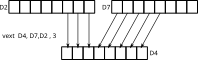
\includegraphics[width=0.56\textwidth]{VEXT.pdf}}
 \end{textblock*} 
%   \begin{lstlisting}[basicstyle=\scriptsize,numbers=none]
%   \end{lstlisting}
\end{frame}

\begin{frame}{NEON General Data Processing Instructions}
 \begin{textblock*}{0.95\textwidth}(0.9cm,1.1cm)
  \begin{itemize}[<+->]\justifying
   \item [VMOV] Rellena un vector con un dato inmediato: I8, I16, I32, I64, F32.
   \item [VMVN] Rellena un vector con la inversa de un dato inmediato: I8, I16, I32, I64, F32.
   \item [VMOVL] Extiende rango. \begin{center}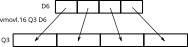
\includegraphics[width=0.5\textwidth]{VMOVL.pdf}\end{center}
   \item [VMOVN] Q Saturation, U Unsigned result. \begin{center}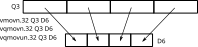
\includegraphics[width=0.5\textwidth]{VMOVN.pdf}\end{center}
   \item [VREV] Vector Reverse Halfword. Permuta las halfwords de cada word de un registro origen y almacena el resultado en un registro destino.
  \end{itemize}
 \end{textblock*}
\end{frame}

\begin{frame}{NEON General Data Processing Instructions}
 \begin{textblock*}{0.95\textwidth}(0.9cm,1.1cm)
  \begin{itemize}[<+->]\justifying
   \item [VSWP] Intercambia los lanes de cada registro destino con los del registro origen
   \item [VTBL] Busca un vector de índices en una tabla y genera un vector de resultados. Los índices fuera de rango retornan 0.
   \item [VTBX] Igual que VTBL excepto que un índice fuera de rango no modifica el elemento del correspondiente vector destino.
   \item [VTRN] Asume sus dos operandos como conformadores de un vector de elementos donde cada elemento es una matriz de 2x2, y simplemente las transpone.\\ 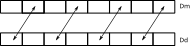
\includegraphics[width=0.5\textwidth]{VTRN.pdf}
  \end{itemize}
 \end{textblock*}
\end{frame}
 
\begin{frame}[fragile]{NEON General Data Processing Instructions}
 \begin{textblock*}{0.95\textwidth}(0.9cm,1.1cm)
  \begin{itemize}\justifying \parskip 0.5 cm
   \item [VUZP] Vector Unzip. Desentrelaza elementos de dos vectores.\\ \vspace{-0.5cm} \begin{center}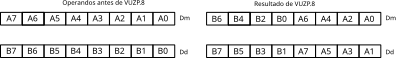
\includegraphics[width=\textwidth]{VUZP.pdf}\end{center}
   \item [VZIP] Vector Zip. Entrelaza los elementos de dos vectores.\\ \vspace{-0.5cm} \begin{center}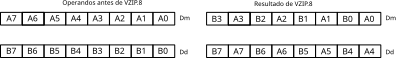
\includegraphics[width=\textwidth]{VZIP.pdf}\end{center}
  \end{itemize}
 \end{textblock*}
\end{frame}

\begin{frame}{NEON Shift Instructions}
 \begin{textblock*}{0.41\textwidth}(1.2cm,1.2cm)
  \begin{itemize}\justifying 
   \item [VSHL] Vector Shift Left. Desplaza a izquierda cada elemento del vector, la cantidad de bits \texttt{\#imm} descartando los bits que salen del elemento por derecha.
   \item [VQSHL] Vector Saturating Shift Left. Setea el bit QC (FPSCR[27]), para indicar que ocurrió una saturación.
   \item [VQSHLU] Vector Saturating Shift Left Unsigned.Setea el bit QC (FPSCR [27]), para indicar que ocurrió una saturación.
  \end{itemize}
 \end{textblock*}
 \begin{textblock*}{.55\textwidth}(.5\textwidth,1.2cm)
  \centering 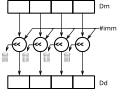
\includegraphics[width=\textwidth]{VSHL.pdf}
 \end{textblock*}
\end{frame}

\begin{frame}{NEON Shift Instructions}
 \begin{textblock*}{\textwidth}(.8cm,1.1cm)
  \begin{itemize}\justifying 
   \item [VSHLL] Vector Shift Left Long. Toma un vector de tamaño doble word, desplaza a izquierda cada elemento del vector, la cantidad de bits \texttt{\#imm} y almacena los resultados en un vector de tamaño Quad Word de la misma cantidad de elementos.
  \end{itemize}
 \end{textblock*}
 \begin{textblock*}{\textwidth}(0.4cm,2.4cm)
  \begin{center}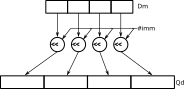
\includegraphics[width=0.5\textwidth]{VSHLL.pdf}\end{center}
 \end{textblock*}
 \begin{textblock*}{\textwidth}(0.4cm,6.5cm)
  \begin{tcolorbox}[enhanced jigsaw,rounded corners, drop fuzzy shadow=ShadowColor]
  Tipos de datos: I8, I16, I32, I64 para VSHL, S8, S16, S32 para VSHLL, VQSHL, o VQSHLU, U8, U16, U32 para VSHLL o VQSHL, S64 para VQSHL o VQSHLU, U64 para VQSHL.
  \end{tcolorbox}
 \end{textblock*}
\end{frame}

\begin{frame}[fragile]{NEON Shift Instructions}
 \begin{textblock*}{.9\textwidth}(1.9cm,1.2cm)
  \begin{itemize}\justifying 
   \item [V\{Q\}\{R\}SHL] Vector Shift Left por variable signada. Desplaza los elementos de un vector en función del número almacenado en los elementos de otro vector. El número puede ser signado (Positivo desplaza a la izquierda, y negativo a la derecha). El resultado se almacena en un tercer registro. Si se emplea la instrución con saturación, se setea el bit QC (FPSCR[27]), para indicar que ocurrió una saturación.
  \end{itemize}
 \end{textblock*}
 \begin{textblock*}{\textwidth}(0.4cm,4.3cm)
 Sintaxis:\vspace{-0.3cm}
  \begin{lstlisting}[basicstyle=\scriptsize,numbers=none]
V{Q}{R}SHL{cond}.datatype {Qd,} Qm, Qn
V{Q}{R}SHL{cond}.datatype {Dd,} Dm, Dn
  \end{lstlisting}
% \vspace{-0.3cm}
\begin{footnotesize}
Q, indica saturación,\\
R Redondeo (si no se especifica, se truncan los resultados)\\
Qd/Dd Registro destino\\
Qm/Dm Registro Operando 1\\
Qn/Dn Registro Operando 2\\
datatype: S8, S16, S32, S64, U8, U16, U32, o U64.\\
\end{footnotesize}
 \end{textblock*}
\end{frame}
   
\begin{frame}{NEON Shift Instructions}
 \begin{textblock*}{0.42\textwidth}(1.2cm,1.2cm)
  \begin{itemize}\justifying 
   \item [VSHR] Vector Shift Right. Desplaza a derecha cada elemento del vector, la cantidad de bits \texttt{\#imm}.
   \item [VRSHR] Idem con redondeo del resultado (Sin la primer R, trunca).
   \item [VSHRN] Idem con Narroewd del resultado (en este caso el primer operando es un registro Q).
   \item [VRSHRN] Idem con redondeo y Narrowed del resultado.
  \end{itemize}
 \end{textblock*}
 \begin{textblock*}{.55\textwidth}(.5\textwidth,1.2cm)
  \begin{center}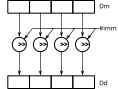
\includegraphics[width=\textwidth]{VSHR.pdf}\end{center}
 \end{textblock*}
\end{frame}

\begin{frame}{NEON Shift Instructions}
 \begin{textblock*}{0.92\textwidth}(1.2cm,1.2cm)
  \begin{itemize}\justifying 
   \item [VSRA] Vector Shift Right and Accumulate. Desplaza a derecha cada elemento del vector, la cantidad de bits \texttt{\#imm} y en lugar de copiarlo al destino se lo acumula.
   \item [VRSRA] Idem con redondeo del resultado (Sin la primer R, trunca).
  \end{itemize}
 \end{textblock*}
 \begin{textblock*}{\textwidth}(0.4cm,2.8cm)
  \begin{center}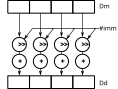
\includegraphics[width=0.45\textwidth]{VSRA.pdf}\end{center}
 \end{textblock*}
\end{frame}

\begin{frame}{NEON Shift Instructions}
 \begin{textblock*}{0.37\textwidth}(1.7cm,1.2cm)
  \begin{itemize}\justifying 
   \item [VQSHRN] Vector Saturating Shift Right Narrow.
   \item [VRQSHRN] Idem con redondeo del resultado.
   \item [VRQSHRUN] Idem con números no signados. 
   \item <2->[VSLI] Vector Shift Left and Insert.
   \item <2->[VSRI] Vector Shift Left and Insert.
  \end{itemize}
 \end{textblock*}
 \begin{textblock*}{.5\textwidth}(.5\textwidth,1.2cm)
  \centering 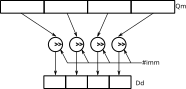
\includegraphics[width=\textwidth]{VQSHRN.pdf}
 \end{textblock*}
\only<2->{
 \begin{textblock*}{.75\textwidth}(.125\textwidth,5.6cm)
  \centering 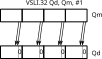
\includegraphics[width=0.45\textwidth]{VSLI.pdf}\hfill
  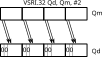
\includegraphics[width=0.45\textwidth]{VSRI.pdf}
 \end{textblock*} 
 }
 \end{frame}

\begin{frame}{NEON logical and compare operations}
 \begin{textblock*}{0.95\textwidth}(0.9cm,1.1cm)
  \begin{itemize}\justifying
   \item [VAND] AND Bitwise entre dos registros. Resultado en el operando destino. Datatype es ignorado.
   \item [VEOR] XOR Bitwise entre dos registros. Resultado en el operando destino. Datatype es ignorado.
   \item [VORR] OR Bitwise entre dos registros. Resultado en el operando destino. O inmediato a registro (\texttt{\#imm}). Datatype es ignorado.
   \item [VORN] OR Bitwise entre dos registros (uno Negado previamente). Resultado en el operando destino. Datatype es ignorado.
   \item [VMVN] Vector Bitwise NOT. Invierte bit a bit el valor del registro Operando en el registro Destino.
   \item [VMOV] Vector Mov. Copia un registro en otro.
   \item [VTST] Vector Test Bits. Ejecuta un AND Bitwise por cada elemento en dos registros. Si el resultado es cero, el elemento correspondiente del operando destino se rellena de '0's. De otro modo se rellena de '1's.
  \end{itemize}
 \end{textblock*}
\end{frame}

\begin{frame}{NEON logical and compare operations}
 \begin{textblock*}{0.95\textwidth}(0.9cm,1.1cm)
  \begin{itemize}\justifying
   \item [VBIC] Vector Bitwise Clear. Dos modos: Inmediato o registro. Inmediato toma el valor inmediato como una máscara. Aquellos bit que están en '1'en la máscara llevan a limpiar (setear '0') en el bit correspondiente del registro resultado. Modo Registro. Operando 1 valos a limpiar, Operando 2 Máscara. Ambos operandos no cambian, ya que se aplica en el registro resultado.
   \item [VBIF] Vector Bitwise Insert if False. Operando 2 trabaja como máscara. Por cada '0' en el Operando 2 el bit correspondiente del Operando 1 reemplaza (se inserta en) al bit correspondiente del resultado, que de otro modo no se altera.
   \item [VBIF] Vector Bitwise Insert if True. Idem anterior pero por cada '1' en Operando 2.
   \item [VBSL] Vector Bitwise Select. El Operando Destino es una máscara. Por cada '1' toma el bit del operando 1 y por cada '0' lo toma del operando 2. El valor compuesto reemplaza la máscara.
  \end{itemize}
 \end{textblock*}
\end{frame}

\begin{frame}{NEON logical and compare operations}
 \begin{textblock*}{0.95\textwidth}(0.9cm,1.1cm)
  \begin{itemize}\justifying
   \item [VACop] Vector Absolute Compare. \texttt{op} puede ser GE = Greater or Equal, o GT = Greater Than. Compara dos vectores Datatype F32 elemento a elemento en valor absoluto. Cada elemento del operando  destino se llena de '1's o '0's, si el par de elementos de los operandos verifica o no la condición. El tipo de dato del resultado es I32.
   \item [VCop] Vector Compare. Compara dos vectores elemento a elemento. La condición \texttt{op}, puede resultar True, en cuyo caso, el elemento destino se completa con '1's, o False, en cuyo caso se completa con '0's.\\
   \texttt{op}: EQ=Equal, GE=Greater or Equal, GT=Greater Than, LE=Lower or Equal, LT=Lower Than. LE y LT valen solo si el segundo operando es \#0.\\
   Trabajan con diferentes tipos de datos tanto los operandos como el resultado de acuerdo con la condición.
  \end{itemize}
 \end{textblock*}
\end{frame}

\begin{frame}{Ejemplo de uso de comparación empaquetada}
 \begin{textblock*}{\textwidth}(0.4cm,1.2cm)
  \Large \centering Procesamiento de sprites o iconos en gráficos 2D. 
  \normalsize
  \begin{itemize}[<+(1)->] \justifying % \parskip 0.2cm
   \item Un sprite es un mapa de bits en el que se dibuja una figura pequeña, de modo tal que los bits que no se utilizan deben quedar \textquotedblleft transparentes", es decir, quedan del color del fondo.
   \item Supongamos un sprite de 8 pixels de ancho por otros 8 pixels de alto. 
   \item Para la primer línea de 8 pixels, el dibujo del sprite corresponde a los primeros cuatro mientras que los cuatro siguientes deben ser transparentes, es decir, deben ir del color del fondo.
   \item Cargamos en \textbf{\texttt{D0}} la primer línea del sprite, (8 bytes empaquetados), y \textbf{\texttt{D2}} trabaja como auxiliar, está pre seteado en cero.
   \item Luego \texttt{\textbf{VCEQ.8}} entre ambos registros, generará una máscara con los bytes que contendrán información del sprite en cero y los que deben resultar transparentes en 0xFF.
  \end{itemize}
 \end{textblock*}
\end{frame}

\begin{frame}{Ejemplo de uso de comparación empaquetada}
 \begin{textblock*}{\textwidth}(0.4cm,1.2cm)
  \centering 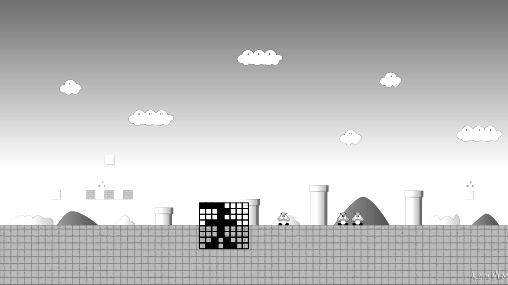
\includegraphics[width=.85\textwidth]{picturebw.pdf}
 \end{textblock*}
\end{frame}

\begin{frame}{Ejemplo de uso de comparación empaquetada}
 \begin{textblock*}{\textwidth}(0.4cm,1.5cm)
  \centering 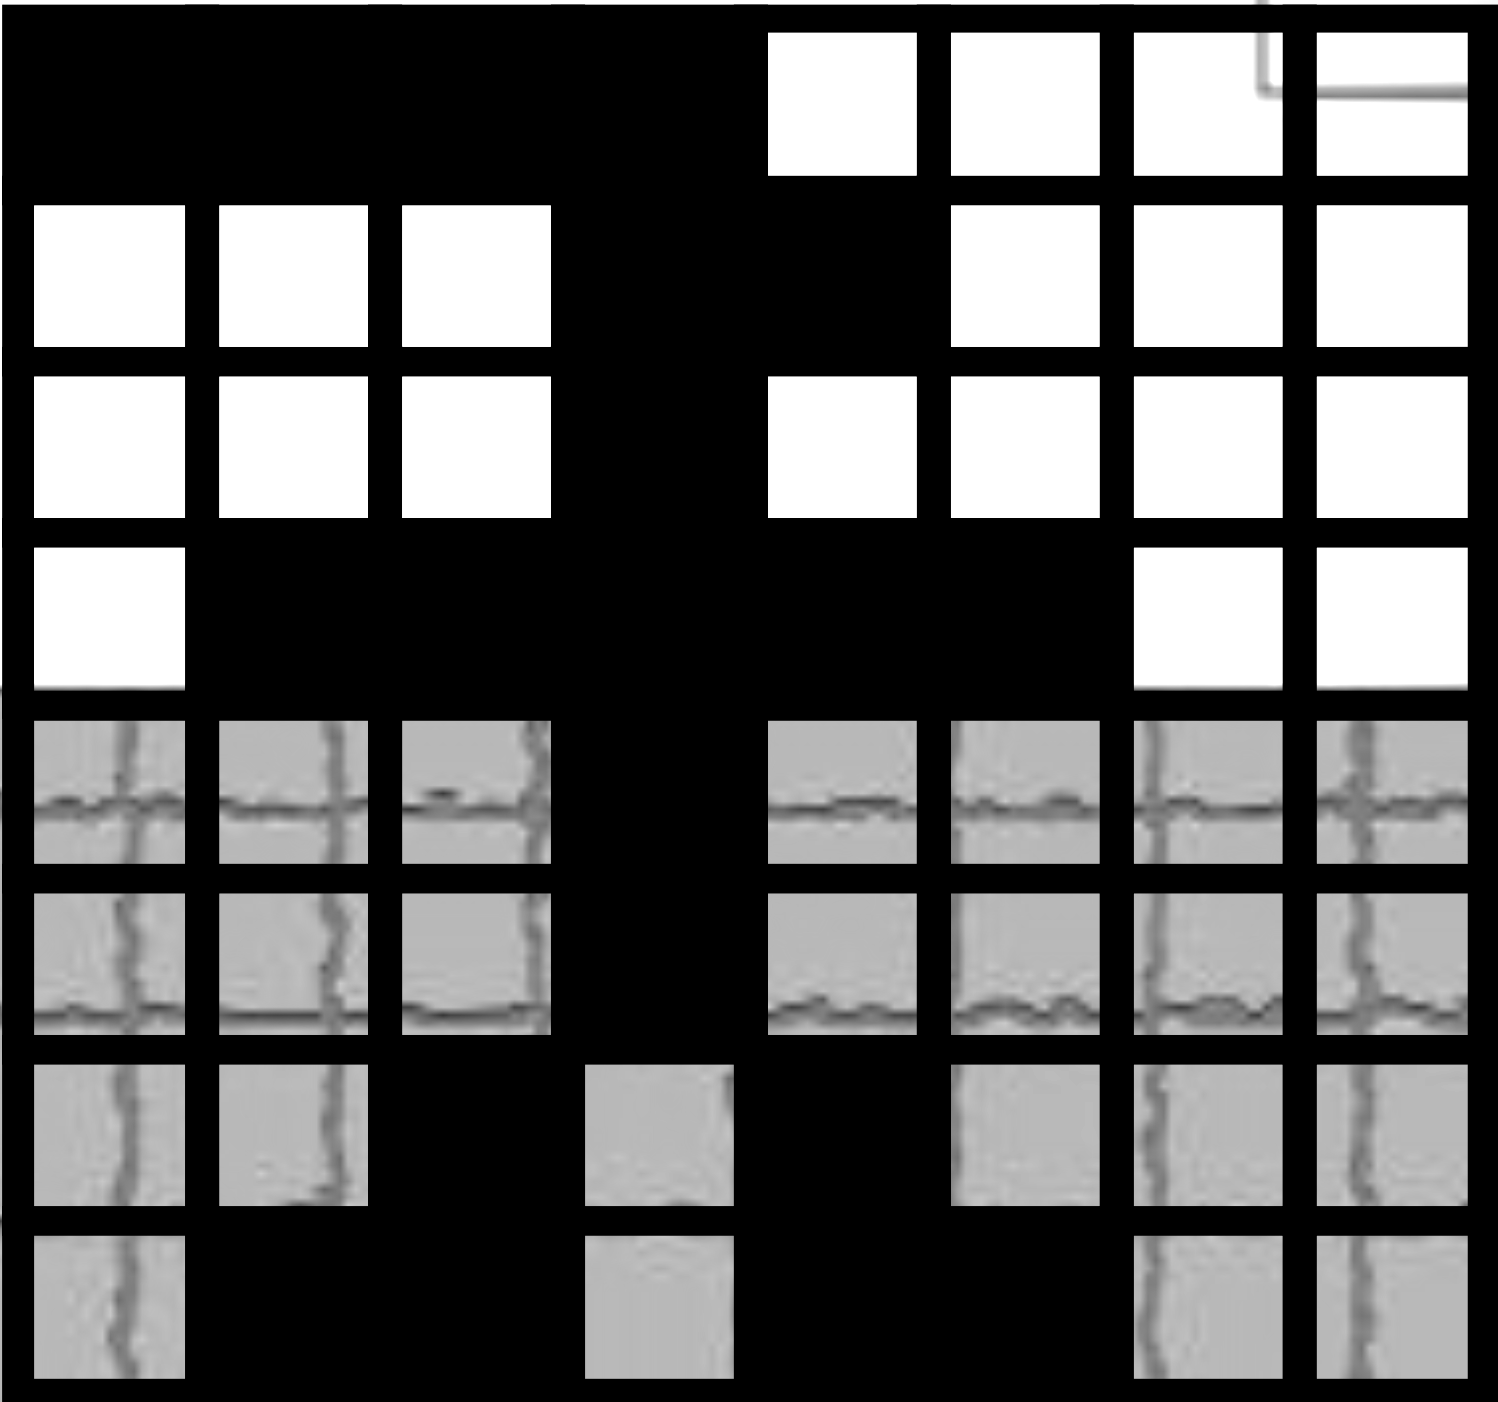
\includegraphics[width=0.47\textwidth]{picture2bw.png}
 \end{textblock*}
\end{frame}

\begin{frame}{Ejemplo de uso de comparación empaquetada}
 \begin{textblock*}{\textwidth}(0.4cm,1.5cm)
  \centering
  \only<1>{\includegraphics[width=0.42\textwidth]{sprite-layer1.pdf} }
  \only<2>{\includegraphics[width=0.42\textwidth]{sprite-layer2.pdf} }
 \end{textblock*}
\end{frame}

\begin{frame}{Ejemplo de uso de comparación empaquetada}
 \begin{textblock*}{0.6\textwidth}(0.1cm,1.2cm)
   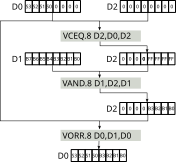
\includegraphics[width=0.8\textwidth]{sprites.pdf}
 \end{textblock*}
\footnotesize
 \begin{textblock*}{0.45\textwidth}(0.1cm+0.56\textwidth,1.2cm)
  \begin{itemize}[<+(1)->] \justifying \parskip 0.2cm
   \item El resultado se procesa con la información de los 8 pixels del fondo de la imagen (pre almacenado en el registro \texttt{\textbf{D1}}) a través de un operador AND. Al resultado le queden solo los cuatro pixels del fondo que se deben mostrar.
   \item Nos queda imprimir la línea del sprite sobre este fondo, del cual hemos eliminado los cuatro pixels que serán sobre impresos por la línea del sprite.
   \item Tratando a este resultado mediante una operación OR con los 8 pixels originales del sprite se compone el dibujo buscado sobre el fondo existente.
  \end{itemize}
 \end{textblock*}
\end{frame}

\begin{frame}{NEON arithmetic instructions}
 \begin{textblock*}{0.95\textwidth}(0.9cm,1.1cm)
  \begin{itemize}\justifying
   \item [VABA] Vector Absolute Difference and Acumulate. Calcula la diferencia entre los elementos de los Vectores de operandos, y acumula el valor absoluto de las mismas en el operando destino. Hay una versión Long.
   \item [VABD] Vector absolute Difference. Idem \textbf{VABA}, pero almacena el valor absoluto de las diferencias en el operando destino. Hay una versión Long.
   \item [VABS] Vector Absolute. Calcula el valor absoluto de los elementos de un vector y almacena su resultado. En el caso de los datatypes de punto flotante simplemente pone '0' en el bit mas significativo. Hay una versión Saturada (VQABS), solo para enteros signados, en donde además se setea el flag QC.
   \item [VADD] Vector Add. Suma los elementos de cada vector de operandos y almacena los resultados en lso elementos correspondientes del Registro destino. Tiene versión es Saturada, Long y Narrow.
  \end{itemize}
 \end{textblock*}
\end{frame}

\begin{frame}{NEON arithmetic instructions}
 \begin{textblock*}{0.9\textwidth}(1.2cm,1.1cm)
  \begin{itemize}\justifying
   \item [VADDHN] Vector Add and Narrow selecting High half. Suma los elementos de los vectores en los registros Operandos, selecciona la mitad alta de los resultados y los almacena en los elementos del vector destino.
   \item [VSUBHN] Vector Subtract and Narrow, selecting High Half. Idem pero Resta.
   \item [VCLS] Vector Count Leading Sign Bits. Cuenta la cantidad de bits consecutivos desde el MSB que coincidan en valor con este y almacena cada cuenta en el elemento correspondiente del registro Destino.
   \item [VCLZ] Vector Count Leading Zeros. Cuenta la cantidad de ceros consecutivos iniciando en el MSB y almacena cada cuenta en el elemento correspondiente del registro Destino.
   \item [VCNT] Vector Count Set Bits. Idem \textbf{VCLZ}, pero cuenta '1's.
  \end{itemize}
 \end{textblock*}
\end{frame}

\begin{frame}{NEON arithmetic instructions}
 \begin{textblock*}{0.9\textwidth}(1.2cm,1.1cm)
  \begin{itemize}\justifying
   \item [VHADD] Vector Halving Add. Suma los elementos de los dos vectores contenidos en los registros operandos, desplaza el resultado a la derecha 1 bit, y almacena cada resultado en el elemento del vector destino. El resultado puede ser redondeado (\textbf{VRHADD}), o truncado.
   \item [VHSUB] Vector Halving Subtract. Idem anterior excepto que resta en lugar de sumar los operandos. No hay redondeo o truncado.
   \item [VMAX] Compara los elementos de dos vectores y almacena en el vector destino el máximo en cada caso.
   \item [VMIN] Compara los elementos de dos vectores y almacena en el vector destino el mínimo en cada caso.
   \item [VNEG] Niega cada elemento de un vector y escribe los resultados en el vector destino. Si el datatyp es Floating Point, invierte el signo. Si el datatype es Entero, dispone de \textbf{VQNEG}, como opción con saturación.
  \end{itemize}
 \end{textblock*}
\end{frame}

%%%%%%%%%%%%%%%%%%%%%%%%%%%%%%%%%%%%%%%%%%%%%%%%%%%%%%%%%%%%%%%%%%%%%%%%
%%%%%%%%%%%%%%%%%%%%%%%%%%%%%%%%%%%%%%%%%%%%%%%%%%%%%%%%%%%%%%%%%%%%%%%%
%%%%%%%%%%%%%%%%%%%%%%%%%%%%%%%%%%%%%%%%%%%%%%%%%%%%%%%%%%%%%%%%%%%%%%%%
%Ejemplo de VMAX y MMIN
%%%%%%%%%%%%%%%%%%%%%%%%%%%%%%%%%%%%%%%%%%%%%%%%%%%%%%%%%%%%%%%%%%%%%%%%
%%%%%%%%%%%%%%%%%%%%%%%%%%%%%%%%%%%%%%%%%%%%%%%%%%%%%%%%%%%%%%%%%%%%%%%%
%%%%%%%%%%%%%%%%%%%%%%%%%%%%%%%%%%%%%%%%%%%%%%%%%%%%%%%%%%%%%%%%%%%%%%%%

\begin{frame}{Ejemplo de procesamiento de imágenes}
 \begin{textblock*}{0.33\textwidth}(0.4cm,1.2cm)
   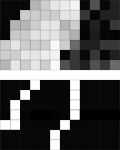
\includegraphics[height=.8\textheight]{Borde-1.pdf}
 \end{textblock*}
 \begin{textblock*}{0.67\textwidth}(0.4cm+0.33\textwidth,1.2cm)
  \begin{itemize}[<+(1)->]\justifying \parskip 0.1cm
   \item Un borde es una transición brusca de iluminación entre dos pixles vecinos.
   \item En el mapa de bits de la izquierda se muestra como queda una imagen resultante de la detección de bordes
   \item Método práctico: por cada pixel tomar los ocho vecinos (N8), y evaluar su diferencia con el mínimo del N8
   \item Si la diferencia es muy grande el valor resultante está próximo al nivel de blanco.
   \item Si ambos valores tienen una diferencia muy pequeña, esta estará próxima al nivel de negro.
   \item Reemplazando cada pixel con la diferencia entre su valor y el MIN(N8), se puede obtener una buena aproximación de los bordes de una imagen
  \end{itemize}
 \end{textblock*}
\end{frame}

\begin{frame}[fragile]{Ejemplo}
 \begin{textblock*}{\textwidth}(0.4cm,1.2cm)
  \begin{tcolorbox}[enhanced jigsaw,rounded corners, drop fuzzy shadow=ShadowColor]
   Supongamos los registros R2, R3, y R4 como punteros a tres áreas de meoria cada una de las cuales contiene una fila de píxeles de una imagen monocromo. Las tres filas son por supuesto consecutivas.
  \end{tcolorbox}
  \begin{onlyenv}<2->
   \lstset{basicstyle=\scriptsize,}
   \vspace{-0.5cm}
   \begin{lstlisting}[escapechar=\@, numbers=none]
// M@\color{Gray}\'e@todo c@\color{Gray}\'a@lculo por N8 
	vldr.u64 {D0-D5},   r2! //q0,q1,q2 primer fila
	vldr.u64 {D6-D11},  r3! //q4,q5,q6 segunda fila 
	//(q5 = lista de pivxeles de inter@\color{Gray}\'e@s)
	vldr.u64 {D12-D17}, r4!	//q7,q8,q9 tercer fila
// Calcula el m@\color{Gray}\'i@nimo de los bytes empaquetados en cada registro
	vmin.U8 Q0,Q0,Q1
	vmin.U8 Q0,Q0,Q2
	vmin.U8 Q0,Q0,Q3
	vmin.U8 Q0,Q0,Q4
	vmin.U8 Q0,Q0,Q6
	vmin.U8 Q0,Q0,Q7
	vmin.U8 Q0,Q0,Q8 
	vmin.U8 Q0,Q0,Q9     //M@\color{Gray}\'i@nimo de los N8 en Q0.
	vsub.U8 Q10,Q5,Q0 //Restamos para hallar los bordes
   \end{lstlisting}
  \end{onlyenv} 
 \end{textblock*}
\end{frame}

%%%%%%%%%%%%%%%%%%%%%%%%%%%%%%%%%%%%%%%%%%%%%%%%%%%%%%%%%%%%%%%%%%%%%%%%
%%%%%%%%%%%%%%%%%%%%%%%%%%%%%%%%%%%%%%%%%%%%%%%%%%%%%%%%%%%%%%%%%%%%%%%%
%%%%%%%%%%%%%%%%%%%%%%%%%%%%%%%%%%%%%%%%%%%%%%%%%%%%%%%%%%%%%%%%%%%%%%%%
%Fin del ejemplo
%%%%%%%%%%%%%%%%%%%%%%%%%%%%%%%%%%%%%%%%%%%%%%%%%%%%%%%%%%%%%%%%%%%%%%%%
%%%%%%%%%%%%%%%%%%%%%%%%%%%%%%%%%%%%%%%%%%%%%%%%%%%%%%%%%%%%%%%%%%%%%%%%
%%%%%%%%%%%%%%%%%%%%%%%%%%%%%%%%%%%%%%%%%%%%%%%%%%%%%%%%%%%%%%%%%%%%%%%%


\begin{frame}{NEON arithmetic instructions}
 \begin{textblock*}{0.45\textwidth}(1.2cm,1.2cm)
  \begin{itemize}\justifying
   \item [VPADD] Vector Pairwise Add. Suma elementos adyacentes de un vector, y escribe resultado en el vector destino.
  \end{itemize}
 \end{textblock*}
 \begin{textblock*}{0.5\textwidth}(0.52\textwidth,1.3cm)
  \centering 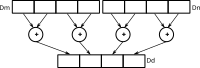
\includegraphics[width=0.8\textwidth]{VPADD.pdf}
 \end{textblock*}
 \begin{textblock*}{0.45\textwidth}(1.2cm,4.0cm)
  \begin{itemize}\justifying
   \item [VPADDL] Vector Pairwise Add Long.
  \end{itemize}
 \end{textblock*}
 \begin{textblock*}{0.5\textwidth}(0.52\textwidth,4.2cm)
  \centering 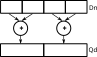
\includegraphics[width=0.4\textwidth]{VPADDL.pdf}
 \end{textblock*}
 \begin{textblock*}{0.45\textwidth}(1.2cm,6.5cm)
  \begin{itemize}\justifying
   \item [VPADAL] Vector Pairwise Add and Accumulate Long.
  \end{itemize}
 \end{textblock*}
 \begin{textblock*}{0.5\textwidth}(0.52\textwidth,6.5cm)
  \centering 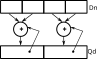
\includegraphics[width=0.4\textwidth]{VPADAL.pdf}
 \end{textblock*}
\end{frame}

\begin{frame}{NEON arithmetic instructions}
 \begin{textblock*}{0.9\textwidth}(1.2cm,1.2cm)
  \begin{itemize}\justifying
   \item [VPMAX] Vector Pairwise Maximum.\\
  \centering 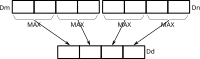
\includegraphics[width=0.45\textwidth]{VPMAX.pdf}
  \end{itemize}
 \end{textblock*}
  \begin{textblock*}{0.9\textwidth}(1.3cm,3.5cm)
  \begin{itemize}\justifying
   \item [VPMIN] Vector Pairwise Maximum. 
   \item [VRECPE] Vector Reciprocal Estimate. Calcula el recíproco estimado de cada elemento de un vector y lo guarda en el vector resultado.
   \item [VRECPS] Vector Reciprocal Step. Multiplica dos vectores elemento a elemento, y resta cada producto de 2.0, y almacena el resultado final en el elemento del vector destino. Es parte de la iteración del algoritmo de Newton-Raphson.
   \item [VRSQRTE] Vector Reciprocal Square Root Estimate. Calcula el recíproco estimado de la raíz cuadrada de cada elemento de un vector y lo guarda en el vector resultado.
  \end{itemize}
 \end{textblock*}
\end{frame}

\begin{frame}{NEON arithmetic instructions}
 \begin{textblock*}{0.9\textwidth}(1.3cm,1.2cm)
  \begin{itemize}\justifying
   \item [VRSQRTS] Vector Reciprocal Square Root Step. Multiplica dos vectores elemento a elemento, resta cada producto de 3.0, y divide cada resultado por 2.0, almacenando en el elemento del vector destino el resultado final. Es parte de la iteración del algoritmo de Newton-Raphson.
   \item [VSUB] Vector Subtract. Resta dos vectores elemento a elemento, y almacena cada resultado en el elemento correspondiente del vector resultado. Tiene versiones saturada (\textbf{VQSUB}), Wide (\textbf{VSUBW}), y Long  (\textbf{VSUBL}).
  \end{itemize}
 \end{textblock*}
\end{frame}

\begin{frame}{NEON Multiply instructions}
 \begin{textblock*}{0.9\textwidth}(1.3cm,1.2cm)
  \begin{itemize}\justifying
   \item [VFMA] Vector Fused Multiply Accumulate. Multiplica dos vectores elemento a elemento, y acumula cada resultado en el elemento correspondiente del vector resultado. No redondea antes de la suma, lo cual la convierte en la alternativa de menor pérdida de precisión.
   \item [VFMS] Vector Fused Multiply Substract. Igual que la anterior, pero resta el resultado del producto de los elementos destino.
   \item [VMUL] Vector Multiply. Multiplica dos vectors elemento a elemento y almacena cada resultado en el correspondiente elemento del vector resultado. Tiene versiones Long ({\color{blue}VMULL}), y escalar.
   \item [VMLA] Vector Multiply Accumulate. Es como \textbf{VFMA} pero redondea antes de la suma.Tiene versiones Long ({\color{blue}VMLAL}) y escalar.
   \item [VMLS] Vector Multiply Substract. Es como \textbf{VFMS} pero redeondea antes de la resta.Tiene versiones Long ({\color{blue}VMLSL}) y escalar.
  \end{itemize}
 \end{textblock*}
\end{frame}

\begin{frame}{NEON Multiply instructions}
 \begin{textblock*}{0.9\textwidth}(1.5cm,1.2cm)
  \begin{itemize}\justifying
   \item [VQDMULH] Vector Saturating Doubling Multiply Returning High Half. Multiplica sus operandos, dupilca los resultados y retorna la parte alta de los mismos. Si ocurrió saturación setea el bit QC. Acepta operar con opción de redondeo (\textbf{VQRDMULH}). Trabaja con vectors y con escalares.
   \item [VQDMULL] Vector Saturating Doubling Multiply Long. Multiplica los operandos y duplica el resultado. Si el resultado da overflow, satura, y setea el bit QC. 
   \item [VQDMLAL] Vector Saturating Doubling Multiply and Accumulate Long. Idem \textbf{VQDMULH}, con el agregado de acumular el  resultado en el destino en lugar de almacenarlo.
   \item [VQDMLSL] Vector Saturating Doubling Multiply and Substract Long. Idem \textbf{VQDMULH}, con el agregado de restar el  resultado en el destino en lugar de almacenarlo.
  \end{itemize}
 \end{textblock*}
\end{frame}

\begin{frame}{NEON Load and Store instructions}
 \begin{textblock*}{\textwidth}(0.4cm,1.2cm)
  \begin{tcolorbox}[enhanced jigsaw,rounded corners, drop fuzzy shadow=ShadowColor]
   Algunas instrucciones Load/Store permiten entrelazar/desentrelazar datos cuando se leen/almacenan estructuras de datos desde/hacia memoria.
  \end{tcolorbox}
  \centering 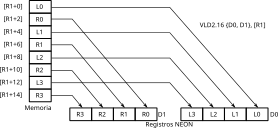
\includegraphics[width=0.8\textwidth]{Interleave.pdf}
 \end{textblock*}
\end{frame}

\begin{frame}[fragile]{NEON Load and Store instructions}
 \begin{textblock*}{\textwidth}(0.4cm,1.5cm)
  \begin{tcolorbox}[enhanced jigsaw,rounded corners, drop fuzzy shadow=ShadowColor]
   Otras instrucciones Load/Store permiten establecer restricciones de alineamiento en memoria.\\
   Para habilitar este chequeo debe setearse el bit SCTLR.A (CP15 System Control Register, bit 1).
  \end{tcolorbox}
  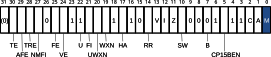
\includegraphics[width=\textwidth]{SCTRL.pdf}
 \end{textblock*}
 \begin{textblock*}{\textwidth}(0.4cm,7cm)
  \begin{onlyenv}<2->
   \begin{lstlisting}[basicstyle=\scriptsize,numbers=none]
MRC p15, 0, R2, c1, c0, 0 # Lee registro SCTRL de CP15 en R2
ORR R2,R2,#0x00000002     # Setea el bit 1 (corresponde a A)
MCR p15, 0, R2, c1, c0, 0 # Activa alineacion escribiendo SCTRL
   \end{lstlisting}
  \end{onlyenv}
 \end{textblock*}
\end{frame}
   
\begin{frame}{NEON Load and Store instructions}
 \begin{textblock*}{\textwidth}(0.4cm,1.5cm)
  \begin{tcolorbox}[enhanced jigsaw,rounded corners, drop fuzzy shadow=ShadowColor]
   A partir de este código cualquier acceso no alineado a memoria genera una \textit{alignment fault}.\\
   Si A=0, no hay restricciones de alineación de memoria, excepto para accesos de ordenamiento estricto o para dispositivos mapeados en memoria (el resultado de un acceso no alineado puede resultar impredecible).
  \end{tcolorbox}
 \end{textblock*}
\end{frame}

\begin{frame}{NEON Load and Store instructions}
 \begin{textblock*}{0.96\textwidth}(0.9cm,1.2cm)
  \begin{itemize}\justifying
   \item [VLDn] Vector Load. \textit{n} puede ser 1, 2, 3, o 4. Carga una estructura de n elementos a uno o mas registros NEON. De acuerdo con la codificación tiene diferentes variantes.
   \begin{itemize}
    \item Cargar un lane en particular de cada registro NEON, y el resto de los lanes no cambian. Utiliza Dd[x] para especificar el lane.
    \item Cargar a todos los lanes de cada registro el mismo dato de la estructura de memoria.
   \end{itemize}
   \item [VSTn] Vector Store. Almacena los lanes de uno o mas registros NEON en una estructura de memoria. Tiene las mismas dos variantes de \textbf{\color{blue}VLDn}.
   \item [VLDR] Carga un Vector de memoria en un registro NEON destino.
   \item [VSTR] Almacena un Registro Neon en n vector de memoria.
  \end{itemize}
 \end{textblock*}
\end{frame}

\begin{frame}{NEON Load and Store instructions}
 \begin{textblock*}{0.95\textwidth}(0.9cm,1.2cm)
  \begin{itemize}\justifying
   \item [VLDM] Carga desde un vector de memoria hacia una lista de uno múltiples registros NEON. Tiene opciones de auto incremento del registro puntero a memoria. Incluye un sufijo de modo:
   \begin{itemize}
    \item IA Increment After (default).
    \item DB Decrement Before.
    \item EA Empty Ascending. Se usa en stacks. Equivale a DB en Loads e IA en Stores.
    \item FD Full Descending. Se usa en stacks. Equivale a IA en Loads e DB en Stores.
   \end{itemize}
   \item [VSTM] Es la operación inversa de {\color{blue}VLDM}. Mismos sufijos y opciones.
   \item [VPOP] Desapila un vector hacia una lista de registros NEON. Equivale a \texttt{VLDM sp!, \{Registros\}}.
   \item [VPUSH] Guarda en la pila un conjunto de registros NEON. Equivale a \texttt{VSTMDB sp! \{Registros\}}.
   \item [VMOV] Mueve datos entre Registros ARM y NEON de 64 bits. Mueve escalares si especificamos el lane en el registro NEON (Dm[x]). 
  \end{itemize}
 \end{textblock*}
\end{frame}

\begin{frame}{NEON Load and Store instructions}
 \begin{textblock*}{.96\textwidth}(0.9cm,1.2cm)
  \begin{itemize}\justifying
   \item [VMRS] Transfiere el registro de sistema NEON o VFP a un registro core (Rn). El regstro de sistema se especifica en la instrucción y puede ser: \textbf{FPSCR}, \textbf{FPSID} , o \textbf{FPEXC}. Detiene el pipeline NEON hasta que se complete su ejecución.
   \item [VMSR] Operación de transferencia inversa a la anterior.
  \end{itemize}
 \end{textblock*}
 \begin{textblock*}{0.96\textwidth}(0.9cm,3.3cm)
  \only <2> {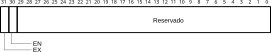
\includegraphics[width=\textwidth]{FPEXC.pdf}\\
  \justifying
  \texttt{\textbf{EX}}. Exception Bit: '0' Indica que el estado NEON y VFP a salvar se compone de los Registros NEON, FPSCR, y FPSID. '1' Indica que hay información adicional implementación específica.\\
  \textbf{\texttt{EN}}. Enable bit. '0' (Default) indica que NEON y VFP no están habilitados. '1' los habilita.\\
  }
  \only <3> {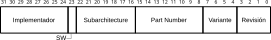
\includegraphics[width=\textwidth]{FPSID.pdf}\\
  \justifying
  \texttt{\textbf{SW}}. '0' Indica que el coprocesador está implementado en hardware. '1' indica que está emulado por software.\\
  }
  \only <4-> {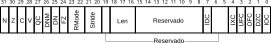
\includegraphics[width=\textwidth]{FPSCR.pdf}\\
  \justifying
  \textbf{\texttt{N}}, \textbf{\texttt{Z}}, \textbf{\texttt{C}} , \textbf{\texttt{V}}, se setean si una comparación resulta \textit{``Menor que''}, \textit{``Igual a''}, \textit{``Mayor a''} o genera un resultado no ordenado, o si produce un resultado no ordenado respectivamente. No actúan hasta que se copien al \textbf{CPSR}.
}
 \end{textblock*}
\end{frame}

\begin{frame}[fragile]{NEON Load and Store instructions}
 \begin{textblock*}{0.45\textwidth}(0.9cm,1.1cm)
   \begin{itemize}\justifying \parskip 0.2cm
   \item [QC] Bit de Saturación
   \item [DNM] Do Not Modify (Reservado)
   \item [DN] Modo NaN. '0' deshabilitado (default). '1' Habilitado.
   \item [FZ] Modo Flush To Zero . '0' deshabilitado. '1' Habilitado.
   \item [RMode] Rounding Mode. '00' Nearest (RN), '01' Hacia $+\infty $ (RP), '10' Hacia $-\infty $ (RM), '11' Hacia Cero (RZ)
  \end{itemize}
 \end{textblock*}
 \begin{textblock*}{0.45\textwidth}(0.55\textwidth,1.1cm)
  \begin{itemize}\justifying \parskip 0.2cm
   \item [Stride] Ver tabla siguiente slide
   \item [Len] Ver tabla siguiente slide
   \item [IDC] Flag de Entrada Denormalizada
   \item [IXC] Flag de Pérdida de precisión
   \item [UFC] Flag de Underflow
   \item [OFC] Flag de Overflow
   \item [DZC] Flag de División por cero
   \item [IOC] Flag de Operación Inválida
  \end{itemize}
 \end{textblock*}
\end{frame}

\renewcommand\theadalign{bc}
\renewcommand\theadfont{\bfseries}
% \renewcommand\theadgape{\Gape[4pt]}
% \renewcommand\cellgape{\Gape[4pt]}

\begin{frame}{NEON Load and Store instructions}
 \begin{scriptsize}
  \begin{center}
   \begin{textblock*}{\textwidth}(0.4cm,1.2cm)
    \begin{tikzpicture}
     \node (tbl) { 
      \rowcolors[]{1}{}{gray!5}
      \begin{tabularx}{.95\textwidth}{ p{.05\textwidth} p{.08\textwidth} p{.05\textwidth} p{.08\textwidth} p{.28\textwidth} p{.27\textwidth} }
       \textbf{\color{white} LEN} & \textbf{\color{white} \thead{Vector\\Length}} & \textbf{\color{white} Stride} & \textbf{ \color{white} \thead{Vector\\Stride} } & \textbf{ \color{white} \thead{SP Vector\\Instructions }} & \textbf{\color{white} \thead{DP Vector\\Instructions}}\\
b000 & 1 & b00 & - & All instructions are scalar & All instructions are scalar\\
b000 & 1 & b11 & - & Unpredictable & Unpredictable\\
b001 & 2 & b00 & 1 & Work normally & Work normally\\
b001 & 2 & b11 & 2 & Work normally & Work normally\\
b010 & 3 & b00 & 1 & Work normally & Work normally\\
b010 & 3 & b11 & 2 & Work normally & Unpredictable\\
b011 & 4 & b00 & 1 & Work normally & Work normally\\
b011 & 4 & b11 & 2 & Work normally & Unpredictable\\
b100 & 5 & b00 & 1 & Work normally & Unpredictable\\
b100 & 5 & b11 & 2 & Unpredictable & Unpredictable\\
b101 & 6 & b00 & 1 & Work normally & Unpredictable\\
b101 & 6 & b11 & 2 & Unpredictable & Unpredictable\\
b110 & 7 & b00 & 1 & Work normally & Unpredictable\\
      \end{tabularx}
     };
     \begin{pgfonlayer}{background}
      \draw[rounded corners,top color=red,bottom color=black,draw=white] ($(tbl.north west)+(0.14,0)$) rectangle ($(tbl.north east)-(0.13,0.9)$);
      \draw[rounded corners,top color=white,bottom color=black, middle color=red,draw=blue!20] ($(tbl.south west)+(0.12,0.15)$) rectangle ($(tbl.south east)-(0.12,0.3)$);
      \draw[top color=blue!1,bottom color=blue!20,draw=white] ($(tbl.north east)-(0.13,0.9)$) rectangle ($(tbl.south west)+(0.13,0.05)$);
%       \draw[top color=blue!1,bottom color=blue!20,draw=white] ($(tbl.north east)-(0.13,0.6)$) rectangle ($(tbl.south west)+(0.13,0.2)$);
     \end{pgfonlayer}
    \end{tikzpicture}
   \end{textblock*} 
  \end{center}
 \end{scriptsize}
\end{frame}



\begin{frame}[t,plain]{Referencias}
\begin{enumerate}
 \item  Una muy buena lectura introductoria (introductoria, o sea para iniciar):
\href{https://developer.arm.com/documentation/dht0002/a}{\textit{\color{blue}\underline{Introducing NEON Development Article}}}

 \vspace {0.8cm}
\item   Referencias Obligadas:

\begin{itemize}
 \item \href{https://developer.arm.com/documentation/den0018/a}{\textit{\color{blue}\underline{NEON Programmer's Guide}}}.

 \item \href{https://documentation-service.arm.com/static/5e8e108088295d1e18d347a5?token=}{\textit{\color{blue}\underline{Cortex-A9 MPCore Technical Reference Manual}}}. Chapter 13. NEON and VFP Programmers Model

 \item \href{https://documentation-service.arm.com/static/5f037ec4dbdee951c1cd73cd?token=}{\textit{\color{blue}\underline{Cortex-A9 NEON Media Processing Engine Technical Reference Manual}}}.

 \item \href{https://developer.arm.com/-/media/Arm\%20Developer\%20Community/PDF/Neon\%20Programmers\%20Guide/102159_0104_01_CodingForNeon.pdf?revision=a3235e10-ded9-4ac8-a415-badcafdd56a6}{\textit{\color{blue}\underline{Coding for Neon}}}.
\end{itemize}

\end{enumerate}

 

 
 



\end{frame}

\end{document}
